\documentclass[11pt,spanish,listoffigures,listoftables]{tfgetsinf}

\usepackage[utf8]{inputenc}
\usepackage{array}
\usepackage{booktabs}
\usepackage{longtable}

\hypersetup{
  colorlinks=true,
  linkcolor=black,
  citecolor=black,
  urlcolor=cyan
}

% El título debe coincidir exactamente con el aprobado por la CAT.
\title{Estudio, adaptación y evaluación de técnicas de superresolución para la mejora de partituras digitalizadas}
\author{Nombre y apellidos del estudiante}
\tutor{Nombre y apellidos del tutor o tutora}
\curs{20XX--20XX}

\keywords
  {superresolució; partitures digitalitzades; processament d'imatge; degradació d'imatge; ajust fi; qualitat d'imatge}
  {superresolución; partituras digitalizadas; procesamiento de imagen; degradación de imagen; ajuste fino; calidad de imagen}
  {super-resolution; digitized music scores; image processing; image degradation; fine-tuning; image quality}

\begin{document}

\chapter*{Agradecimientos}
\addcontentsline{toc}{chapter}{Agradecimientos}

Agradezco conjuntamente a Elena Vázquez Barrachina, tutora del TFG, y a Jorge Calvo Zaragoza,
director experimental, su orientación, acompañamiento y contribución al desarrollo integral de
este trabajo. Agradezco asimismo a la Societat Joventut Musical d'Albal la autorización para
acceder y procesar el material utilizado en la prueba profesional externa. Este TFG no ha recibido
financiación externa.


\begin{abstract}[spanish]
La baja resolución de una partitura digitalizada puede deteriorar pentagramas, símbolos, dígitos y
texto. La superresolución permite generar una imagen de mayor tamaño, pero los modelos entrenados
con imágenes naturales pueden producir detalles visualmente plausibles que no estaban presentes en
el documento. Este Trabajo de Fin de Grado estudia cuándo estas técnicas aportan valor y qué
precauciones exige su uso profesional en bibliotecas, archivos, conservación, consulta o
preparación editorial.

Se auditó Sheet Music Benchmark (SMB) y se reservó una muestra intacta para la comparación
principal. Esta utilizó 64 páginas de 64 grupos documentales y seis degradaciones sintéticas:
factores de ampliación dos y cuatro, combinados con severidad limpia, moderada y fuerte. Para que la
severidad fuese comparable entre páginas, el desenfoque se normalizó por la separación entre líneas
de pentagrama. Se compararon interpolación bicúbica, la red residual EDSR y el transformador ligero
SwinIR mediante PSNR y SSIM sobre luminancia, intervalos emparejados por grupo, tiempo de inferencia
y una revisión cualitativa preseleccionada de errores de notación. La implementación reproducible
se desarrolló en Python con PyTorch, OpenCV y \texttt{uv}, y la ejecución acelerada se realizó en
Kaggle sobre GPU Tesla T4.

Tras preservar la comparación principal, se ejecutó un estudio secundario de ajuste fino de EDSR.
Se definieron roles internos con 45 grupos de entrenamiento, 13 de validación y 20 de
prueba, sin solapamiento de identificadores ni reutilización de los 64 grupos principales.
Estos grupos pueden ser movimientos de una misma composición: no garantizan independencia
musical y los intervalos son descriptivos, condicionados a esa agrupación. El modelo adaptado superó al
EDSR oficial en PSNR-Y y SSIM-Y para las seis condiciones, con intervalos emparejados que no
cruzaron cero. Este resultado respalda adaptación sobre documentos retenidos de SMB con degradaciones
coincidentes, sin certificar generalización a composiciones nunca vistas ni corrección musical.

Como extensión profesional, el modelo adaptado se aplicó sin reajuste a doce obras de un archivo
musical externo bajo las mismas degradaciones. Los intervalos favorecieron al modelo adaptado en
las seis comparaciones PSNR-Y y en cinco de seis SSIM-Y. Ocho derivados se aceptaron para consulta,
tres con reservas y uno se rechazó; también se implementó un demostrador local reversible. Esta
prueba respalda transferencia entre colecciones bajo LR sintética, no restauración de entradas LR
naturales ni una tasa universal de seguridad.

EDSR y SwinIR superaron a bicúbica en las dos métricas primarias para las seis condiciones. Sin
embargo, SwinIR solo mejoró claramente a EDSR en las condiciones x2 limpia, x2 moderada y x4 limpia,
y fue entre 5,2 y 8,5 veces más lento. La revisión visual detectó símbolos alterados, corrupción de
texto y trazos curvos o texturados incluso cuando aumentaba la fidelidad promedio. Se concluye que
EDSR ofrece el compromiso más defendible entre fidelidad y coste para generar copias de consulta
asistidas, mientras que SwinIR debe reservarse para condiciones donde su ganancia compense el
coste. Ningún método queda validado como restauración semántica, sustituto archivístico o entrada
autónoma de OMR: debe conservarse el original y someterse cada derivado relevante a revisión humana.

\end{abstract}

\begin{abstract}[catalan]
La baixa resolució d'una partitura digitalitzada pot deteriorar pentagrames, símbols, dígits i
text. La superresolució permet generar una imatge més gran, però els models entrenats amb imatges
naturals poden produir detalls visualment plausibles que no estaven presents en el document. Aquest
Treball de Fi de Grau estudia quan aquestes tècniques aporten valor i quines precaucions exigeix el
seu ús professional en biblioteques, arxius, conservació, consulta o preparació editorial.

Es va auditar Sheet Music Benchmark (SMB) i es va reservar una mostra intacta per a la comparació
principal. Aquesta va utilitzar 64 pàgines de 64 obres independents i sis degradacions
sintètiques: factors d'ampliació dos i quatre, combinats amb severitat neta, moderada i forta. Perquè
la severitat fora comparable entre pàgines, el desenfocament es va normalitzar per la separació
entre línies de pentagrama. Es van comparar la interpolació bicúbica, la xarxa residual EDSR i el
transformador lleuger SwinIR mitjançant PSNR i SSIM sobre luminància, intervals aparellats per obra,
temps d'inferència i una revisió qualitativa preseleccionada d'errors de notació. La implementació
reproduïble es va desenvolupar en Python amb PyTorch, OpenCV i \texttt{uv}, i l'execució accelerada
es va realitzar en Kaggle sobre GPU Tesla T4.

Després de preservar la comparació principal, es va executar un estudi secundari d'ajust fi
d'EDSR. Es van definir rols interns per obra amb 45 grups d'entrenament, 13 de validació i 20 de
prova, sense solapament ni reutilització de les 64 obres principals. El model adaptat va superar
l'EDSR oficial en PSNR-Y i SSIM-Y per a les sis condicions, amb intervals aparellats que no van
creuar zero. Aquest resultat demostra adaptació dins d'SMB i degradacions coincidents, no
transferència a altres col·leccions ni correcció musical.

Com a extensió professional, el model adaptat es va aplicar sense reajustar-lo a dotze obres d'un
arxiu musical extern sota les mateixes degradacions. Els intervals van afavorir el model adaptat en
les sis comparacions PSNR-Y i en cinc de sis SSIM-Y. Huit derivats es van acceptar per a consulta,
tres amb reserves i un es va rebutjar; també es va implementar un demostrador local reversible.
Aquesta prova dona suport a la transferència entre col·leccions sota LR sintètica, no a la
restauració d'entrades LR naturals ni a una taxa universal de seguretat.

EDSR i SwinIR van superar la interpolació bicúbica en les dues mètriques primàries per a les sis
condicions. No obstant això, SwinIR només va millorar clarament EDSR en les condicions x2 neta, x2
moderada i x4 neta, i va ser entre 5,2 i 8,5 vegades més lent. La revisió visual va detectar símbols
alterats, corrupció de text i traços corbs o amb textura fins i tot quan augmentava la fidelitat
mitjana. Es conclou que EDSR ofereix el compromís més defensable entre fidelitat i cost per a generar
còpies de consulta assistides, mentre que SwinIR s'ha de reservar per a les condicions on el guany
compense el cost. Cap mètode queda validat com a restauració semàntica, substitut arxivístic o
entrada autònoma d'OMR: cal conservar l'original i verificar humanament cada derivat rellevant.

\end{abstract}

\begin{abstract}[english]
Low resolution can damage staff lines, symbols, digits, and text in a digitized music score.
Super-resolution can generate a larger image, but models trained on natural images may introduce
visually plausible detail that was not present in the document. This Bachelor's Thesis studies
when these techniques add value and which safeguards are required for professional use in
libraries, archives, preservation, consultation, or editorial preparation.

Sheet Music Benchmark (SMB) was audited and an untouched sample was reserved for the primary
comparison. It used 64 pages from 64 documentary groups and six synthetic degradations: two
and four times upscaling crossed with clean, moderate, and strong severity. Blur was normalized by
staff-line spacing so that severity remained comparable across pages. Bicubic interpolation, the
EDSR residual network, and lightweight SwinIR were compared using luminance PSNR and SSIM,
paired intervals by group, inference time, and a preselected qualitative review of notation
failures. The reproducible implementation was developed in Python with PyTorch, OpenCV, and
\texttt{uv}; GPU execution used one Tesla T4 device on Kaggle.

After preserving the primary comparison, a secondary EDSR fine-tuning study was performed.
Project-defined roles comprised 45 training, 13 validation, and 20 test groups, with no identifier
overlap or reuse of the 64 primary groups. Groups can be movements of the same composition:
musical independence is not guaranteed, and intervals are descriptive and conditional on this
grouping. Adapted EDSR exceeded the official model in luminance PSNR and SSIM under all six
conditions, with group-paired intervals that did not cross zero. This supports adaptation on
held-out SMB documents under matched degradations, without certifying generalization to unseen
complete compositions or musical correctness.

As a professional extension, the adapted model was applied without retuning to twelve works from
an external music archive under the same degradations. Intervals favored the adapted model in all
six PSNR comparisons and five of six SSIM comparisons. Eight derivatives were accepted for
consultation, three with reservations, and one was rejected; a reversible local demonstrator was
also implemented. This supports cross-collection transfer under synthetic LR, not restoration of
naturally acquired LR inputs or a universal safety rate.

EDSR and SwinIR outperformed bicubic interpolation on both primary metrics in all six conditions.
However, SwinIR clearly exceeded EDSR only for x2 clean, x2 moderate, and x4 clean inputs, while
requiring 5.2 to 8.5 times more inference time. Visual review found altered symbols, corrupted text,
and curved or textured strokes even when average fidelity improved. EDSR therefore provides the
most defensible fidelity--cost trade-off for assisted access copies, whereas SwinIR should be
reserved for conditions in which its additional gain justifies the cost. None of the evaluated
methods is validated as semantic restoration, an archival replacement, or an autonomous input to
optical music recognition. The original must be retained and every consequential derivative must
be checked by a human reviewer.

\end{abstract}

\chapter*{Glosario y abreviaturas}
\addcontentsline{toc}{chapter}{Glosario y abreviaturas}

\emph{Pendiente: mantener esta sección solo si la versión final utiliza abreviaturas o términos
técnicos que necesiten una definición previa. Ordenar alfabéticamente y emplear las mismas formas
en toda la memoria.}


\mainmatter

\chapter{Introducción}

\section{Motivación y problema profesional}
La digitalización permite consultar y preservar colecciones musicales, pero una resolución
insuficiente puede degradar líneas de pentagrama, cabezas y plicas de nota, alteraciones, texto y
otros elementos pequeños. La superresolución puede mejorar la legibilidad aparente de estas
imágenes, aunque una reconstrucción visualmente convincente no garantiza que conserve la
información musical. El problema profesional de este TFG es, por tanto, determinar cuándo y cómo
puede utilizarse esta técnica sin introducir cambios plausibles pero musicalmente significativos.

Los destinatarios principales son profesionales de digitalización, bibliotecas, archivos,
conservación y patrimonio musical. Como usuarios secundarios se consideran intérpretes,
investigadores y editoriales. Para todos ellos, la utilidad de una técnica dependerá no solo de la
calidad visual, sino también de la fidelidad de la notación, el coste computacional, las licencias
y las condiciones concretas de uso.

La elección del problema combina interés formativo y relevancia aplicada. Permite integrar visión
por computador, aprendizaje profundo, tratamiento de datos y evaluación estadística en un objeto
con estructura semántica exigente. A diferencia de una fotografía natural, una variación mínima
puede cambiar una alteración, un dígito o la continuidad de una línea. Esta propiedad convierte la
partitura en un caso especialmente útil para aprender a distinguir mejora visual, fidelidad y
seguridad de uso. El trabajo cuenta con la orientación conjunta de Elena Vázquez Barrachina y
Jorge Calvo Zaragoza; el diseño, la implementación, la revisión de resultados y las conclusiones
son responsabilidad del autor.

\section{Objetivo general y objetivos específicos}
El objetivo general es evaluar un conjunto pequeño y científicamente contrastado de técnicas de
superresolución sobre degradaciones controladas de partituras digitalizadas, medir su fidelidad,
coste y errores de notación, y convertir la evidencia en un marco de decisión por método,
degradación y uso profesional. Una conclusión válida puede ser que ningún método resulte adecuado
para una condición determinada.

Los objetivos específicos son:
\begin{itemize}
  \item construir un estado del arte trazable basado en fuentes primarias y oficiales;
  \item auditar e inventariar de forma inmutable el conjunto SMB y preservar una muestra
        confirmatoria intacta para la comparación principal;
  \item predeclarar degradaciones, comparadores, unidades independientes, resultados y límites de
        interpretación antes de observar resultados finales;
  \item comparar los métodos sobre entradas emparejadas mediante evidencia de fidelidad, recursos
        y fallos específicos de notación;
  \item evaluar una adaptación acotada con obras separadas de la muestra confirmatoria y sin
        consultar la prueba durante el entrenamiento;
  \item comprobar, sin reajuste posterior, la transferencia del modelo adaptado a una colección
        externa mediante un piloto profesional y un demostrador local reversible; y
  \item producir recomendaciones profesionales reproducibles y limitadas a la evidencia obtenida.
\end{itemize}

Estos objetivos se concretan en seis preguntas de evaluación:
\begin{enumerate}
  \item ¿qué diferencia de PSNR-Y y SSIM-Y presenta cada red respecto de bicúbica dentro de cada
        combinación predeclarada de escala y severidad?;
  \item ¿cambia la relación entre EDSR y SwinIR al aumentar la escala o la severidad?;
  \item ¿qué defectos de pentagramas, símbolos, texto o textura aparecen en los casos cualitativos
        fijados y cuál es su origen observable: entrada degradada, reconstrucción o falta de
        recuperación?;
  \item ¿qué compromiso existe entre fidelidad, tiempo de inferencia, licencias y riesgo de uso?; y
  \item ¿mejora un ajuste fino acotado de EDSR la fidelidad sobre obras SMB no vistas, manteniendo
        separadas las funciones de entrenamiento, validación y prueba?; y
  \item ¿mantiene ese modelo su ventaja al aplicarse, sin reajuste, a obras de otra colección bajo
        las mismas degradaciones sintéticas, y resultan sus salidas utilizables como copias de
        consulta?
\end{enumerate}
No se formuló una hipótesis nula única ni se aplicó un contraste confirmatorio global. Los
intervalos emparejados cuantifican incertidumbre descriptiva sobre comparaciones predeclaradas;
la relevancia profesional requiere además magnitud, evidencia cualitativa y coste.

\section{Impacto esperado y alcance}
La contribución obtenida es una guía de decisión que identifica condiciones de uso, límites y
casos en los que no debe recomendarse la superresolución. Incluye una comparación principal de
modelos preentrenados, un estudio secundario de adaptación dentro de SMB y, tras asegurar ambos, un
piloto sobre doce obras de una colección externa acompañado de un demostrador local de imágenes.
Las conclusiones quedan restringidas a las poblaciones, métodos y degradaciones controladas
realmente evaluadas. El piloto permite estudiar transferencia entre colecciones bajo LR sintética,
pero no demuestra restauración de entradas de baja resolución adquiridas naturalmente. Quedan
fuera la reconstrucción de PDF, el reconocimiento óptico de música y el despliegue público.

\section{Metodología}
El estudio siguió un enfoque de contrato primero. Antes de la evaluación final se fijaron la identidad
del conjunto de datos, las unidades independientes, el manifiesto, los operadores de degradación,
los comparadores, las métricas, el muestreo cualitativo y las reglas de interpretación. La muestra
principal SMB no se empleó para elegir modelos, puntos de control, hiperparámetros ni umbrales. El
estudio secundario congeló antes de entrenar roles por obra sin solapamiento y excluyó las 64 obras
de la comparación principal. El piloto externo fijó después sus doce obras, seis condiciones,
comparadores y casos de revisión antes de generar ninguna salida. Las páginas reciben entradas
idénticas para todos los comparadores y se agrupan por obra o fuente auditada, mientras que las
regiones se tratan como observaciones anidadas.

La evaluación combinó medidas de fidelidad con una revisión sistemática de discontinuidades de
pentagrama, pérdida o deformación de símbolos, uniones indebidas, alteraciones de texto y marcas
alucinadas. También se registró el tiempo de inferencia y el entorno de ejecución. Cada afirmación
material se vinculó a evidencia revisada, con denominador y limitaciones explícitos.

\section{Estructura de la memoria}
Tras esta introducción, el capítulo 2 sintetiza el estado del arte y delimita la brecha; el capítulo
3 analiza alternativas, restricciones y riesgos; y el capítulo 4 documenta los datos y su gobierno.
Los capítulos posteriores describen metodología, resultados, validación profesional, conclusiones
y trabajo futuro. Los anexos conservarán la información de reproducibilidad y, al final, la
reflexión sobre los Objetivos de Desarrollo Sostenible compartida con su entrega independiente.

\chapter{Estado del arte}

\section{Superresolución de imágenes}
La interpolación cúbica constituye una referencia transparente para reconstruir muestras sobre una
rejilla de mayor resolución, pero su formulación no demuestra por sí misma fidelidad en partituras
\cite{keys1981cubic}. % Claim evidence: SOTA-INTERPOLATION-ROLE
Por ello, este trabajo conservará las interpolaciones vecina, bilineal y bicúbica como comparadores
simples, no como soluciones cuya idoneidad se presuponga.

La superresolución convolucional introdujo una correspondencia aprendida de extremo a extremo y
los modelos residuales posteriores ampliaron esa familia orientada a la fidelidad
\cite{dong2015srcnn,lim2017edsr}. Sus resultados publicados proceden principalmente de imágenes
naturales degradadas de forma sintética; sirven para definir familias de comparación, pero no se
transfieren como resultados sobre SMB ni seleccionan un modelo para este TFG.
% Claim evidence: SOTA-CNN-FOUNDATION

Los enfoques adversariales mostraron que una imagen percibida como más realista puede obtener peores
medidas de distorsión, y la literatura formalizó el compromiso entre percepción y distorsión
\cite{ledig2017srgan,blau2018perception,wang2018esrgan}.
% Claim evidence: SOTA-PERCEPTION-DISTORTION
Este compromiso es especialmente relevante en notación musical: generar un detalle verosímil no
equivale a recuperar el símbolo presente en la fuente. Los transformadores de restauración, como
SwinIR y HAT, amplían el contexto modelado y presentan avances en bancos de imágenes naturales
\cite{liang2021swinir,chen2023hat}; su progresión arquitectónica tampoco decide todavía la
implementación ni los pesos que se estudiarán en la fase experimental.
% Claim evidence: SOTA-TRANSFORMER-PROGRESSION

La literatura reciente incorpora además superresolución generativa de un solo paso y controles del
equilibrio entre fidelidad y realismo \cite{kim2026fidesr,zhang2026tadsr}. En paralelo, el trabajo
sobre texto de escena introduce guías estructurales de glifos \cite{luo2026tiger}. Los resultados
publicados en esos dominios justifican examinar el riesgo semántico, pero no establecen seguridad
para símbolos musicales ni compatibilidad ejecutable con este estudio.
% Claim evidence: SOTA-CURRENT-GENERATIVE-RISK

\section{Restauración de documentos y partituras}
La restauración documental abarca problemas que no son equivalentes a la superresolución, como
descurvado, eliminación de sombras, binarización o mezclas de degradaciones
\cite{zhang2024docres,li2026mmdir}. Un estudio de superresolución de escaneos documentales muestra
además que la fidelidad alineada y el beneficio para reconocimiento de texto pueden evolucionar de
forma distinta \cite{zyrek2025document}. Estas fuentes motivan controles de geometría y de tarea,
pero no demuestran la conservación de la notación musical.
% Claim evidence: SOTA-DOCUMENT-SCOPE

Existe trabajo primario directamente orientado a superresolución de partituras, evaluado sobre
DeepScores con una red residual normalizada por instancia \cite{tran2019scoresr}. El conjunto Sheet
Music Benchmark (SMB) aporta un contexto oficial posterior para la evaluación de reconocimiento
óptico de música y de errores sobre elementos musicales \cite{martinez2025smb}. Esta evidencia no
convierte las métricas de reconocimiento en métricas de superresolución ni prueba que la búsqueda
enfocada sea exhaustiva.
% Claim evidence: SOTA-DIRECT-SCORE-EVIDENCE

También debe separarse la degradación sintética controlada de la degradación real. SwinIR estudia
tareas clásicas y reales, mientras que Real-ESRGAN utiliza una cadena sintética de degradación de
orden alto y el trabajo documental de Zyrek et al. emplea escaneos registrados
\cite{liang2021swinir,wang2021realesrgan,zyrek2025document}. Cada configuración responde a una
pregunta distinta; sus resultados no pueden agruparse como una única validación.
% Claim evidence: SOTA-DEGRADATION-BOUNDARY

\section{Evaluación y brecha identificada}
El estado del arte muestra que PSNR, SSIM y medidas perceptuales describen propiedades
complementarias, no una noción única de calidad. En partituras debe añadirse evidencia sobre
continuidad de pentagramas, geometría de símbolos, elementos pequeños, uniones o separaciones
indebidas, texto y marcas musicalmente significativas. Las mejoras publicadas en imágenes naturales,
documentos o reconocimiento no bastan para responder a esas preguntas.

La brecha abordada por este TFG es una evaluación trazable que combine fidelidad emparejada,
fallos específicos de notación, recursos y condiciones profesionales. La contribución no será un
ranking universal de modelos, sino un marco condicionado por método, degradación y uso, con límites
y casos de no recomendación. La selección exacta de modelos, repositorios, licencias y puntos de
control se actualizará antes de la fase de comparación; no queda fijada por esta revisión inicial.

\chapter{Análisis del problema y solución propuesta}

\section{Restricciones, alternativas y decisión}
Una comparación útil debe distinguir tres niveles: interpolaciones simples, un conjunto pequeño de
modelos preentrenados con papeles científicos diferentes y, únicamente si la validación lo
justifica, una adaptación acotada. Se descarta recopilar muchos modelos sin profundidad analítica y
también se descarta convertir una aplicación, el tratamiento de PDF o el reconocimiento óptico de
música en requisito del núcleo experimental.

La solución aplicada fue una comparación controlada y reproducible sobre entradas emparejadas,
seguida de una adaptación secundaria de EDSR. La comparación principal permaneció intacta; para la
adaptación se asignaron otros grupos de fuente SMB a roles de entrenamiento, validación y prueba
sin solapamiento de páginas ni identificadores. Esta separación operativa no garantiza independencia
entre composiciones completas, pues distintos grupos pueden corresponder a movimientos de una
misma obra. Una vez asegurados ambos estudios se admitió una extensión acotada: un demostrador
local y una prueba sin reajuste sobre obras externas. Cada comparación compartió condiciones y
reglas de agregación dentro de su propio denominador, y la interpretación integró fidelidad,
errores de notación, recursos, licencias y restricciones operativas.
La Tabla~\ref{tab:alternatives} resume las opciones consideradas y la razón por la que cada una se
incorporó, aplazó o excluyó.

\begin{table}[htbp]
  \centering
  \footnotesize
  \setlength{\tabcolsep}{3pt}
  \caption{Alternativas valoradas antes de cerrar el alcance. Fuente: elaboración propia.}
  \label{tab:alternatives}
  \begin{tabular}{p{0.20\textwidth}p{0.23\textwidth}p{0.24\textwidth}p{0.23\textwidth}}
    \toprule
    Alternativa & Valor que aportaba & Coste o amenaza & Decisión \\
    \midrule
    Bicúbica únicamente & Referencia rápida y explicable & No representa un método aprendido & Incluir como línea base, no como única solución \\
    EDSR y SwinIR preentrenados & Dos familias y pesos oficiales para x2/x4 & Transferencia desde imágenes naturales & Incluir y auditar fallos musicales \\
    Modelos perceptuales o difusión & Mayor realismo aparente & Alucinación, más coste y menor trazabilidad & Excluir del núcleo orientado a fidelidad \\
    Ajuste fino & Posible adaptación al dominio & Riesgo de fuga y coste adicional & Ejecutar un estudio secundario acotado tras asegurar el núcleo \\
    Demostrador y piloto externo & Evidencia tangible de aplicabilidad & Nueva pregunta, derechos y revisión adicional & Ejecutar una extensión acotada después de asegurar el núcleo \\
    PDF, OMR o despliegue & Flujo de producto o tarea posterior & Validación y riesgos distintos & Mantener como trabajo futuro \\
    \bottomrule
  \end{tabular}
\end{table}

\section{Riesgos técnicos y científicos}
El primer riesgo era la contaminación del benchmark: inspeccionar resultados, ajustar umbrales o
seleccionar modelos con la muestra principal de SMB habría invalidado su papel de evaluación final.
El control adoptado mantuvo
el conjunto bloqueado hasta congelar manifiesto, métodos, puntos de control, degradaciones,
métricas, exclusiones, muestreo y reglas de interpretación.

Otros riesgos fueron la desalineación entre entrada y referencia, la pérdida de denominadores por
errores de procesado y la falsa precisión al tratar páginas o regiones de una misma obra como
observaciones independientes. Se conservaron los fallos explícitos, se verificó el emparejamiento
y se agrupó por identificador de fuente SMB. Este control no elimina la posible dependencia entre
movimientos o ediciones relacionados, que limita la interpretación de los intervalos.

Los métodos perceptuales y generativos pueden producir detalle visualmente plausible sin garantizar
su correspondencia con la fuente \cite{ledig2017srgan,wang2018esrgan,kim2026fidesr}.
% Claim evidence: SOTA-PERCEPTION-DISTORTION, SOTA-CURRENT-GENERATIVE-RISK
Por ello, una mejora agregada no bastó: se revisaron pentagramas, símbolos, dígitos y texto, y se
retuvieron también ejemplos negativos. Los riesgos de tiempo, memoria y energía se registraron por
ejecución y justificaron detener extensiones opcionales antes de comprometer el núcleo o el margen
de entrega.
La matriz de la Tabla~\ref{tab:risk-matrix} conecta estos riesgos con sus controles y con el
resultado realmente observado, incluido el fallo del primer protocolo de degradación.

\begin{table}[htbp]
  \centering
  \footnotesize
  \setlength{\tabcolsep}{3pt}
  \caption{Riesgos principales, controles aplicados y resultado. Fuente: elaboración propia a
  partir del registro de riesgos del proyecto.}
  \label{tab:risk-matrix}
  \begin{tabular}{p{0.22\textwidth}p{0.10\textwidth}p{0.10\textwidth}p{0.29\textwidth}p{0.19\textwidth}}
    \toprule
    Riesgo & Prob. & Impacto & Control & Resultado \\
    \midrule
    Contaminar la prueba & Media & Crítico & Congelación previa y separación por ID de fuente; 64 grupos principales excluidos de la adaptación & Sin IDs compartidos; dependencia entre movimientos no descartada \\
    Degradación no transferible & Media & Crítico & Calibración visual y trazas por página & Ocurrió en v1; corregido y repetido como v2 \\
    Métricas favorables con error musical & Media & Crítico & Revisión cualitativa fija y regla de contradicción & Ocurrió en casos; limita la recomendación \\
    Peso, licencia o entorno incompatible & Media & Alto & Fuentes oficiales, hashes y prueba Kaggle & Resuelto antes de la ejecución final \\
    Coste o plazo excesivo & Alta & Crítico & Núcleo primero y extensión acotada a EDSR & Controlado; se preservó la evaluación \\
    Derechos por imagen insuficientes & Media & Alto & Separar acceso, procesamiento y reproducción; documentar base, atribución y proporcionalidad & Comparaciones seleccionadas; la autorización del archivo no acredita todos los derechos \\
    \bottomrule
  \end{tabular}
\end{table}

\section{Marco legal, ético y medioambiental}
La documentación oficial de SMB informa de acceso controlado y licencia CC BY-NC 4.0
\cite{martinez2025smb,smbDatasetCard,ccByNc40}, pero esa etiqueta no se interpretó automáticamente
como autorización ilimitada para redistribuir cualquier escaneo o transformación. Deben separarse
la licencia del conjunto, la procedencia y derechos de cada partitura, las licencias del código y
los pesos, y la base que permite publicar cada figura. La memoria utiliza SMB con atribución,
finalidad académica no comercial e indicación de las transformaciones; reproduce recortes y una
única comparación de página completa elegida de antemano porque resulta necesaria para explicar el
comportamiento global del sistema. El resto del conjunto y los paneles completos no se
redistribuyen. La reproducción se integra en el análisis y juicio crítico, identifica la obra y la
fuente y se limita a la extensión justificada por ese propósito. El artículo 32.1 de la
Ley de Propiedad Intelectual \cite{boeLpiArticle32} se considera como base de cita y análisis,
sujeta a sus requisitos en cada reproducción. No se presupone que la licencia del conjunto
resuelva por sí sola todos los derechos de cada edición o digitalización.

En el piloto externo, la Societat Joventut Musical d'Albal (SJMA) autorizó el acceso, procesamiento
y reproducción en el TFG de las doce páginas de prueba aportadas. La memoria muestra el conjunto
cualitativo externo completo ---ocho casos aceptados, tres con reservas y un rechazo--- como
fragmentos instrumentales de obras de banda, vinculados directamente a comparaciones y comentarios
críticos. Se atribuyen obra, autor
o arreglista, parte e institución de procedencia; no se publican las otras cuatro páginas recibidas,
el corpus bruto ni las restantes salidas. La autorización institucional y este uso analítico
acotado no se describen como cesión ni
como titularidad del estudiante sobre las obras, arreglos o ediciones. La custodia del archivo y
su autorización no acreditan por sí solas todos los derechos de reproducción pública de terceros;
la base aplicable debe valorarse para cada imagen, especialmente en las páginas completas.

La evaluación consideró como amenazas las representaciones insuficientes de fuentes, estilos de grabado,
densidades de notación, tamaños de pentagrama, tipografías y calidades de digitalización. También se
evitaron afirmaciones de beneficio universal o de reconocimiento no medido. El principal riesgo
ético es presentar una reconstrucción inventada como documento fiel, con posibles consecuencias
para consulta, interpretación, edición o conservación. El análisis medioambiental registró
hardware, duración y consumo computacional pertinente en lugar de asumir que un modelo más complejo
es profesionalmente preferible.

No se trataron datos personales ni se entrenó un sistema de decisión sobre personas, por lo que no
se identificó un tratamiento de categorías personales ni un riesgo de discriminación individual.
Sí existe un sesgo documental: solo se estudió notación impresa compatible con SMB y la selección
final exigió una escala de pentagrama mensurable. El piloto añadió partes de banda de otra
colección, pero no manuscritos, tradiciones de notación no representadas, entradas LR naturales
heterogéneas ni páginas que el estimador no pudo caracterizar. La consecuencia ética no es asignar
un resultado a una persona, sino ofrecer peor cobertura o una falsa
sensación de fidelidad para determinados documentos.

\section{Plan de trabajo y recursos}
El trabajo se organiza en incrementos de evidencia: contrato y gobierno de SMB; degradaciones e
interpolaciones; selección y validación de modelos; evaluación controlada; y síntesis, reproducción
y depósito. El núcleo científico tuvo prioridad; solo después de reconciliarlo se añadieron la
adaptación acotada de EDSR y, como última extensión separable, el piloto externo con demostrador
local. El tratamiento de PDF, OMR, despliegue, nuevas familias y mejoras no esenciales permanecen
fuera del alcance. La contingencia final se reserva para comentarios de los
revisores, correcciones invalidantes, reproducción limpia y operaciones de depósito.

La planificación inicial asignó 330 horas al TFG. Al no existir un parte horario contemporáneo,
se realizó una reconstrucción retrospectiva por paquetes de trabajo, contrastada con los hitos,
artefactos, ejecuciones y revisiones conservados. La estimación de referencia, anterior al piloto
externo y a las tareas finales de cierre, es
de 346 horas, con un intervalo prudente de 312 a 380 horas. La distribución central fue de 64 horas
para el contrato, el estado del arte y el gobierno de SMB; 73 para el diseño experimental y las
líneas base; 71 para integrar los modelos y ejecutar la adaptación acotada; 82 para las dos ejecuciones SMB,
la corrección del protocolo y el análisis; y 56 para la memoria y su control de calidad. Se estiman
22 horas adicionales para incorporar las dos revisiones, cerrar el depósito y preparar la defensa,
lo que situó la previsión previa en 368 horas. El piloto profesional recibió después una envolvente
adicional de 10--16 horas, de modo que la previsión final pasa a 378--384 horas sin atribuir como
dedicación del estudiante el tiempo de cómputo no supervisado. Estas cifras
expresan dedicación académica estimada, no una medición cronográfica, y por ello se comunica también
su incertidumbre.
La Figura~\ref{fig:effort} contrasta la distribución por fases con el plan inicial; sus barras
cubren esa estimación de referencia, mientras que la previsión final de
378--384 horas incorpora también el cierre y el piloto profesional.

Frente al plan, la evaluación consumió más por detectar que la primera degradación no se transfería
a páginas completas, normalizarla por la escala del pentagrama y repetir el experimento. La
adaptación secundaria añadió unas 20 horas una vez protegido el núcleo. Antes del piloto, la
previsión aumentaba 38 horas (un 11,5\,\%) respecto de las 330 iniciales y rebasaba en 8 horas el
límite superior del intervalo orientativo de 300--360 horas asociado a los 12 ECTS; la extensión
eleva la diferencia prevista a 48--54 horas. Se comunica la desviación en lugar de ajustar
retrospectivamente el esfuerzo al intervalo. Los recursos materiales fueron el equipo local ya
disponible, Overleaf y una GPU gratuita de Kaggle; no se imputa un coste salarial ficticio ni un
gasto no documentado.

\begin{figure}[htbp]
  \centering
  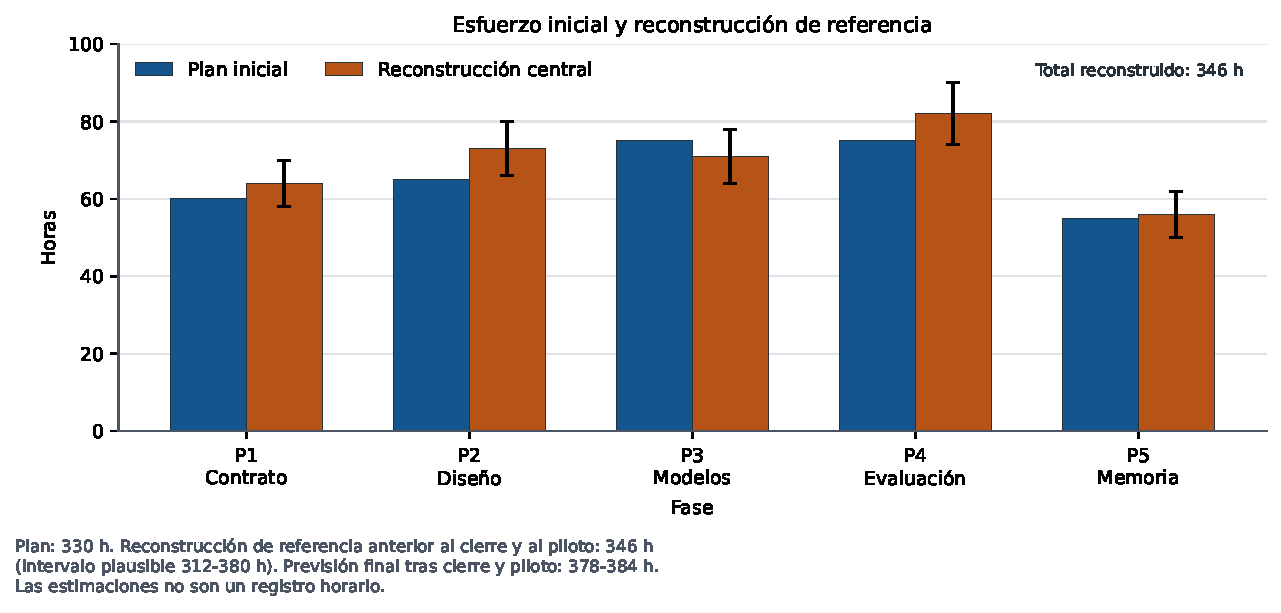
\includegraphics[width=\textwidth]{figures/context/effort-plan-vs-reconstruction.pdf}
  \caption{Comparación entre el plan inicial y la reconstrucción retrospectiva por fase. Las barras
  de error expresan el intervalo plausible, no variabilidad estadística; la figura cubre 346 horas
  centrales de referencia, no las 378--384 horas previstas tras el cierre y el piloto.
  Fuente: elaboración propia a partir del registro de esfuerzo.}
  \label{fig:effort}
\end{figure}

\begin{table}[htbp]
  \centering
  \small
  \caption{Recursos y costes directos planificados. Fuente: elaboración propia.}
  \label{tab:resources-cost}
  \begin{tabular}{p{0.27\textwidth}p{0.37\textwidth}p{0.22\textwidth}}
    \toprule
    Recurso & Uso & Coste incremental \\
    \midrule
    Equipo local disponible & Desarrollo, auditoría, pruebas y análisis & 0 € de adquisición; 20--80 € estimados de electricidad y red \\
    Kaggle con Tesla T4 & Inferencia aprendida acotada & 0 € en el plan ejecutado \\
    Overleaf y TeX Live local & Edición autoritativa y prevalidación & 0 € incremental \\
    Almacenamiento y copias & Datos restringidos y artefactos fuera de Git & 0--30 € de contingencia \\
    Impresión y trámites & Solo si el proceso vigente lo exige & 0--50 € provisionales \\
    \midrule
    Total externo & Rango de planificación; no gasto acreditado & 20--160 € \\
    \bottomrule
  \end{tabular}
\end{table}

La Tabla~\ref{tab:resources-cost} separa la dedicación académica de los costes directos externos.
El trabajo del estudiante se expresa en horas y no se monetiza con una tarifa inventada. Del mismo
modo, disponer de una cuota gratuita no equivale a coste ambiental nulo: al no medirse energía, el
análisis se limita a duración, hardware y decisiones de reducción de cálculo.

\chapter{Preparación y comprensión de los datos}

\section{Procedencia, licencia y versión}
El conjunto principal de evaluación es Sheet Music Benchmark (SMB), publicado como
\texttt{PRAIG/SMB}. La auditoría utiliza la revisión inmutable
\texttt{96332e8c4ac8\ldots}. Su artículo y ficha oficial informan de
685 páginas de notación musical impresa, acceso manualmente controlado, una única partición oficial
\texttt{test} y licencia del conjunto CC BY-NC 4.0
\cite{martinez2025smb,smbDatasetCard,ccByNc40}.
% Claim evidence: SOTA-DIRECT-SCORE-EVIDENCE
% Source revision: 96332e8c4ac81cbdb7f61093ec5a4bfff76a0adb
% Resolver of record: proyecto/data/manifests/smb-evaluation-v1.yaml
% Selected recovery descriptor:
% proyecto/data/manifests/recovery/canonical-pixel-v2/
% c8d62c14724b38e1c4a415db503a689dad87f0ce9308cf0121a3fe9bd688f69f/manifest-recovery.yaml
El manifiesto activo y recuperable es la generación de contenido direccionado
\allowbreak{\footnotesize\texttt{d97ac77f7ee672fca2c3d09b8d6fbf319719306d4ed8315e9cf8b56ec373e3fe}}, cuyos registros
tienen SHA-256
\allowbreak{\footnotesize\texttt{56cebb344ae512a3dea16ce4848bce197f971493c98c5c388fe9a094922b820b}}. La procedencia de
la ejecución vincula de forma determinista la revisión limpia del código de auditoría, su árbol de
fuentes y \texttt{uv.lock}. La recuperación sin conexión verifica los hashes, los contratos, la
concordancia de la procedencia embebida y la identidad de la generación antes de materializarla;
no reconstruye por sí sola el repositorio ni \texttt{uv.lock}. Como comprobación separada, una
verificación automatizada independiente del pipeline principal reconstruyó desde el commit limpio
registrado los mismos digests del árbol de fuentes, del parche vacío y del fichero de bloqueo.

La licencia y el acceso están confirmados en el nivel del conjunto, pero la procedencia por elemento
no está disponible. En el manifiesto congelado, la redistribución no queda establecida y la
reproducción de figuras permanece prohibida como estado operativo preventivo por defecto. Ese
registro histórico no se reescribió después de observar los resultados. Una decisión de
publicación posterior y separada limitó la excepción a una selección atribuida de recortes y una
comparación de página completa, necesaria para explicar el problema y analizar críticamente
entradas y salidas. Se indica la transformación, se mantiene la finalidad académica no comercial y
no se presenta SMB como un corpus libre de restricciones.

El acceso controlado y la licencia obligan a separar reproducibilidad y redistribución. Las imágenes
fuente, los paneles no seleccionados y los pesos adaptados derivados de SMB se conservan fuera de
Git; solo se publican dentro de la memoria las composiciones analíticas identificadas.

\section{Auditoría, cobertura y calidad}
% Evidence: proyecto/data/manifests/smb-evaluation-v1.yaml and the recovery bundle selected by it;
% human decisions: proyecto/data/audits/smb-visual-sample-v1.csv and smb-review-v1.csv
La auditoría automatizada conserva las 685 filas del inventario y todas se procesaron. De ellas,
618 tienen anotaciones válidas y son elegibles para análisis emparejados que dependan
de las anotaciones; las 67 restantes permanecen en el denominador, pero son inelegibles para ese
contrato: 66 contienen al menos una región sin alguno de los textos obligatorios
\texttt{raw}, \texttt{kern} o \texttt{ekern}
(\texttt{missing\_required\_region\_text}) y una presenta una caja regional fuera del dominio
porcentual permitido (\texttt{invalid\_region\_}\allowbreak\texttt{annotation}). La validación admite únicamente una
tolerancia numérica de \(10^{-9}\) puntos porcentuales para ruido de representación. La
superresolución de página completa no consume esos textos, por lo que esta bandera no fue un
criterio de exclusión del experimento de imagen. La política de agrupación humana revisada asigna
el inventario a 260 grupos documentales sin contar las páginas de un mismo identificador como
observaciones independientes. Hay 619 páginas con textos completos: una de ellas falla por su caja
regional y, por tanto, no pertenece al grupo de 618 anotaciones válidas.

La revisión visual humana se limitó a 64 páginas seleccionadas mediante una regla fijada antes de
cualquier resultado. Las otras 621 páginas no se revisaron visualmente de forma individual. Dentro
del alcance de esa muestra no se observaron incidencias materiales de calidad o idoneidad; esta
observación no permite atribuir la misma valoración a las 685 páginas ni estimar su prevalencia en
toda la población.

La comparación criptográfica no produjo ningún par exacto. Se conservaron 14 pares candidatos por
hash perceptual y la revisión humana los clasificó como distintos, sin eliminarlos del inventario.
La generación auditada permaneció en estado \texttt{AUDITED\_LOCKED}. La autorización final no
modificó ese inventario: un registro separado vinculó previamente métodos, puntos de control,
degradaciones, métricas, muestra y reglas de interpretación, y únicamente entonces permitió la
evaluación v2.

La Tabla~\ref{tab:smb-audit-summary} distingue el inventario auditado de la muestra confirmatoria.
Esta separación evita presentar los 64 grupos documentales evaluados como si representaran automáticamente las
685 páginas o las 260 fuentes del conjunto.

\begin{table}[htbp]
  \centering
  \small
  \setlength{\tabcolsep}{3pt}
  \caption{Cobertura de la auditoría y de la evaluación final de SMB. Fuente: elaboración propia a
  partir del manifiesto auditado.}
  \label{tab:smb-audit-summary}
  \begin{tabular}{p{0.25\textwidth}p{0.14\textwidth}p{0.52\textwidth}}
    \toprule
    Evidencia & Cantidad & Interpretación \\
    \midrule
    Páginas inventariadas y procesadas & 685 & Denominador completo del conjunto auditado \\
    Anotaciones válidas & 618 & Elegibles para análisis que dependan de la anotación \\
    Anotaciones no válidas & 67 & Se conservan; 66 por texto ausente y una por caja inválida \\
    Grupos documentales & 260 & Unidad operativa por identificador; no equivale a composición completa \\
    Muestra visual de auditoría & 64 & Calidad e idoneidad revisadas; no estima prevalencia en las 685 páginas \\
    Pares candidatos perceptuales & 14 & Revisados como distintos; no eliminados \\
    Candidatas al recorrido v2 & 427 páginas / 207 grupos & Tras excluir los 53 grupos de v1 y las relaciones duplicadas o pendientes \\
    Rechazos de escala antes del cierre v2 & 76 de 140 examinadas & 75 procedían del grupo de 618 y una del grupo de 67 \\
    Muestra confirmatoria v2 & 64 páginas / 64 grupos & 56 del grupo de 618 y ocho del de 67; todas con escala mensurable \\
    \bottomrule
  \end{tabular}
\end{table}

La Figura~\ref{fig:smb-profile} caracteriza el inventario sin reproducir sus imágenes. Las 685
páginas se reparten entre 260 grupos documentales: 132 aportan una sola página, mientras que el grupo mayor aporta
14. Las dimensiones varían entre 900 y 2.550 píxeles de anchura y entre 277 y 3.289 de altura, y el
número de regiones anotadas va de 1 a 12, con mediana 6. Los clústeres visibles de resolución
sugieren procesos de generación o captura diferenciados; esta observación describe el corpus, pero
no identifica por sí sola equipos, épocas o calidad.

\begin{figure}[htbp]
  \centering
  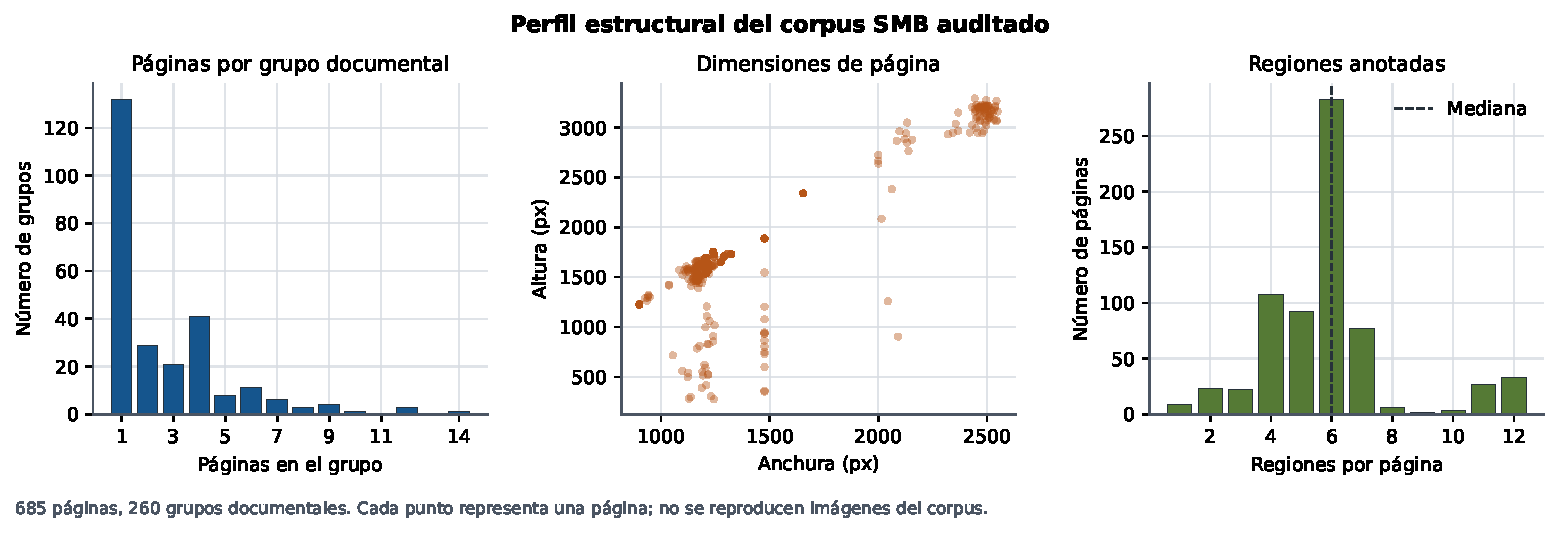
\includegraphics[width=\textwidth]{figures/context/smb-dataset-profile.pdf}
  \caption{Perfil de páginas por grupo documental, dimensiones y regiones anotadas en el inventario completo.
  Fuente: elaboración propia a partir de 685 registros del manifiesto SMB.}
  \label{fig:smb-profile}
\end{figure}

El recorrido desde el conjunto hasta la muestra final se resume en la
Figura~\ref{fig:sample-flow}. No partió exclusivamente de las 618 páginas con anotaciones
válidas, ya que la reconstrucción de página completa no utiliza esos campos. Tras excluir los 53
grupos del piloto v1 y las páginas con relaciones duplicadas o pendientes, quedaron 427 candidatas
de 207 grupos documentales. El recorrido determinista examinó 140 páginas hasta reunir 64 grupos documentales: el estimador
descartó 76 por no poder establecer una escala válida, 75 de ellas pertenecientes al grupo de 618
y una al grupo de 67. Las 64 aceptadas comprenden 56 páginas del primer grupo y ocho del segundo;
estas ocho conservaban píxeles y geometría aptos para la evaluación, aunque les faltara algún texto
regional no usado por los modelos ni por las métricas. La selección de una página por grupo evita
repetir un identificador y facilita la comparación, pero introduce un sesgo de mensurabilidad que debe acompañar
a cualquier conclusión.

\begin{figure}[htbp]
  \centering
  \begin{tikzpicture}[
      node distance=6mm,
      box/.style={draw, rounded corners=2pt, align=center, minimum width=0.82\textwidth,
        minimum height=8mm, fill=blue!5},
      arrow/.style={-{Latex[length=2mm]}, thick}]
    \node[box] (all) {685 páginas procesadas en 260 grupos documentales\\
      618 con anotación válida y 67 con anotación no válida};
    \node[box, below=of all] (candidates) {427 páginas candidatas de 207 grupos documentales\\
      tras excluir grupos v1 y relaciones duplicadas o pendientes};
    \node[box, below=of candidates] (scale) {140 páginas examinadas hasta el cierre\\
      76 rechazadas por escala: 75 del grupo de 618 y una del de 67};
    \node[box, below=of scale, fill=green!8] (sample) {64 páginas de 64 grupos documentales\\
      56 del grupo de 618 y ocho del de 67};
    \draw[arrow] (all) -- (candidates);
    \draw[arrow] (candidates) -- (scale);
    \draw[arrow] (scale) -- (sample);
  \end{tikzpicture}
  \caption{Flujo de selección del inventario a la muestra confirmatoria. Fuente: elaboración
  propia a partir del manifiesto y de la selección congelada.}
  \label{fig:sample-flow}
\end{figure}

\section{Particiones y prevención de fugas}
\label{sec:smb-grouping}
SMB solo publica una partición oficial denominada \texttt{test}; las etiquetas de entrenamiento,
validación y prueba utilizadas en este TFG son, por tanto, roles internos y no nuevas particiones
oficiales. En la comparación principal, los 64 grupos documentales de la muestra v2 se reservaron íntegramente
para inferencia: no se utilizaron para entrenamiento, validación, ajuste de hiperparámetros,
elección de métodos o puntos de control.

La unidad operativa fue el grupo documental identificado por \texttt{source\_group\_id},
obtenido de \texttt{original\_score} al retirar únicamente el sufijo de página \texttt{\_pN}.
Un grupo puede corresponder a un documento, un movimiento o una sección, y no equivale
necesariamente a una composición completa. Las páginas se evaluaron de forma emparejada y las
regiones o recortes se trataron como observaciones anidadas. El manifiesto reconcilió los índices
esperados y comprobó la separación de páginas e identificadores entre roles; en la muestra
principal se retuvo una página por grupo. Esta comprobación no acredita la independencia musical
entre todos los grupos.

Por ejemplo, \texttt{beethoven\_sonata01\_2} aparece en entrenamiento (índices 339--341) y
\texttt{beethoven\_sonata01\_4} en prueba (390--396, con representante 391);
\texttt{mozart\_sonata15\_1} aparece en entrenamiento (652--654) y
\texttt{mozart\_sonata15\_3} en prueba (578). Son movimientos de las mismas sonatas
distribuidos entre roles distintos. No se constató reutilización de las mismas páginas o píxeles,
pero persiste dependencia potencial entre movimientos, secciones o ediciones. Por ello, los
resultados SMB describen documentos retenidos y no certifican generalización a composiciones
completas nunca vistas. No se realizó un análisis de sensibilidad por composición completa;
los manifiestos y resultados congelados se conservan sin redefinir retrospectivamente sus grupos.

El estudio secundario de adaptación se definió después de cerrar aquella comparación, pero antes
de entrenar o consultar sus resultados. Excluyó los 64 grupos documentales v2; asignó al entrenamiento 45 grupos documentales
del piloto v1, con 212 páginas elegibles; y seleccionó entre grupos no utilizados 13 para validación y 20
para prueba, con 35 y 55 páginas elegibles. La selección de punto de control empleó 13 casos fijos
de validación, mientras que la prueba utilizó una página representativa por cada uno de sus 20
grupos. Ningún identificador de grupo cruzó roles y los identificadores de validación y prueba no
habían aparecido en v1 ni v2. Esta separación permite estudiar adaptación dentro del corpus con
documentos distintos de la comparación principal, con la dependencia residual indicada; no
demuestra independencia por composición ni transferencia a otra colección.
La Tabla~\ref{tab:adaptation-split} hace explícitos los tres roles internos y sus denominadores.

\begin{table}[htbp]
  \centering
  \small
  \caption{Roles internos del estudio secundario de adaptación EDSR. No son particiones oficiales
  de SMB. Fuente: elaboración propia a partir del manifiesto congelado.}
  \label{tab:adaptation-split}
  \begin{tabular}{lrrp{0.39\textwidth}}
    \toprule
    Rol & Grupos & Páginas elegibles & Uso \\
    \midrule
    Entrenamiento & 45 & 212 & Muestreo equilibrado de recortes; grupos del piloto v1 \\
    Validación & 13 & 35 & Selección de punto de control sin consultar prueba \\
    Prueba & 20 & 55 & Una página fija por grupo y seis condiciones \\
    \bottomrule
  \end{tabular}
\end{table}

\section{Corpus externo para la prueba profesional}
La prueba de transferencia empleó páginas aportadas por el archivo musical de la Societat Joventut
Musical d'Albal (SJMA), ajenas a SMB. La entidad autorizó el acceso, el procesamiento y la
reproducción de una selección en este trabajo; el estudiante compiló el corpus, pero no se atribuye
la titularidad de las obras, arreglos o ediciones subyacentes. Las páginas HR, LR y reconstruidas
permanecen fuera de Git y no se distribuyen como colección. La memoria reproduce las doce
comparaciones cualitativas predeclaradas, atribuidas y comentadas, para hacer auditables todos los
veredictos y no solo los resultados favorables. Esta autorización acotada no se presenta como permiso
general de publicación o explotación de las partituras.

Se recibieron dieciséis partes de banda de una página. Antes de generar resultados, tres se
asignaron exclusivamente a ingeniería del estimador de pentagrama y una quedó como reserva por
redundancia de sus características de entrada. Las doce restantes, una por obra independiente, se
congelaron como prueba externa. La selección utilizó únicamente tipo de fuente, orientación,
instrumento, densidad, estado documental, presencia de texto y escala estimada; no consultó ninguna
salida de superresolución.

\begin{table}[htbp]
  \centering
  \small
  \caption{Composición del corpus externo congelado. Fuente: elaboración propia a partir del
  manifiesto privado de la SJMA.}
  \label{tab:external-corpus}
  \begin{tabular}{lp{0.27\textwidth}p{0.43\textwidth}}
    \toprule
    Rol & Cantidad & Cobertura de entrada \\
    \midrule
    Ingeniería & 3 obras & Casos usados para corregir el estimador; excluidos de resultados \\
    Prueba & 12 obras & 10 fuentes digitales y 2 escaneos; 8 verticales y 4 horizontales \\
    Reserva & 1 obra & Excluida por redundancia antes de observar salidas \\
    \bottomrule
  \end{tabular}
\end{table}

Entre las doce obras de prueba había siete páginas de notación densa, tres media y dos dispersa;
todas contenían texto. La separación estimada entre líneas de pentagrama abarcó de 10 a 15 píxeles
HR, con mediana 12,75. Las dimensiones variaron entre 1.818 y 2.572 píxeles de anchura y entre 1.818
y 2.629 de altura. Estas propiedades amplían la variedad documental respecto de SMB, pero doce
partes de banda no representan todas las colecciones profesionales.
La composición y las exclusiones previas del corpus se sintetizan en la
Tabla~\ref{tab:external-corpus}.

\section{Degradación controlada}
La evaluación final utilizó el protocolo \texttt{staff-scale-score-v2}. Se mantuvieron seis
condiciones, correspondientes a los factores de ampliación \(\times 2\) y \(\times 4\) y a los
perfiles \emph{clean}, \emph{moderate} y \emph{strong}. En todas ellas la reducción se efectuó con
\texttt{INTER\_AREA}. El perfil limpio no añadió ninguna operación posterior. En el perfil
moderado, el desenfoque gaussiano se definió como
\(\max(0{,}3,0{,}05s)\) píxeles de la imagen de alta resolución, donde \(s\) es la separación
entre líneas de pentagrama; tras la reducción se añadió ruido gaussiano acromático con
\(\sigma=1{,}5\) y compresión JPEG de calidad 80 sin submuestreo de crominancia. En el perfil
fuerte se emplearon \(\max(0{,}3,0{,}15s)\), \(\sigma=2{,}5\) y calidad JPEG 45,
respectivamente. La semilla maestra fue 20260830 y cada aplicación conservó sus parámetros y su
semilla efectiva.
La Tabla~\ref{tab:degradation-v2} permite reproducir los operadores y distingue el perfil limpio de
los dos niveles que añaden desenfoque, ruido y compresión.

\begin{table}[htbp]
  \centering
  \small
  \caption{Operadores del protocolo de degradación final. \(s\) es la separación entre líneas de
  pentagrama medida en la imagen HR. Fuente: elaboración propia.}
  \label{tab:degradation-v2}
  \begin{tabular}{lccc}
    \toprule
    Perfil & Desenfoque gaussiano HR & Ruido tras reducción & JPEG 4:4:4 \\
    \midrule
    Limpio & ninguno & ninguno & ninguno \\
    Moderado & \(\max(0{,}3;0{,}05s)\) & gaussiano acromático, \(\sigma=1{,}5\) & calidad 80 \\
    Fuerte & \(\max(0{,}3;0{,}15s)\) & gaussiano acromático, \(\sigma=2{,}5\) & calidad 45 \\
    \bottomrule
  \end{tabular}
\end{table}

La Figura~\ref{fig:degradation-profiles} traduce estos parámetros a su efecto visual. Se aplica la
misma escala \(\times 4\) y el mismo recorte HR en los tres perfiles: así, las diferencias no se
deben a la obra ni al contenido elegido. La entrada limpia pierde resolución por el submuestreo;
la moderada añade una pérdida visible pero conserva las estructuras principales; y la fuerte hace
más inciertas las alteraciones, separaciones internas y líneas finas. Las LR se amplían por vecino
más próximo solo para compararlas al mismo tamaño, no como método de reconstrucción.

\begin{figure}[htbp]
  \centering
  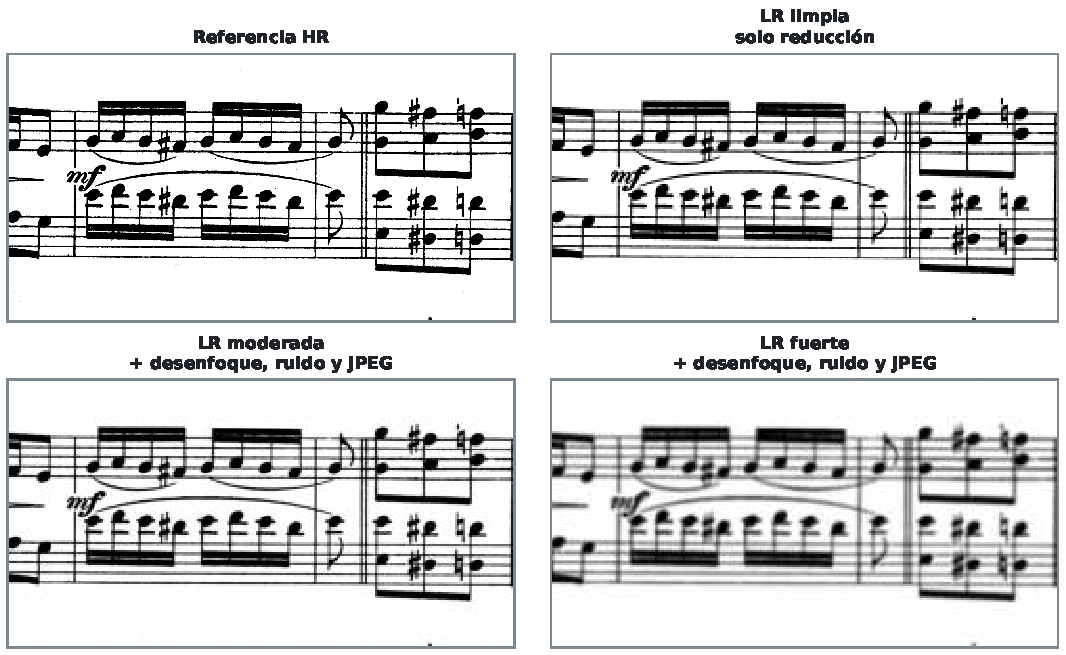
\includegraphics[width=\textwidth]{figures/context/degradation-profiles-x4.pdf}
  \caption[Ejemplo visual de los tres perfiles de degradación]{Efecto de los perfiles limpio,
  moderado y fuerte a escala \(\times 4\) sobre el mismo fragmento. La versión moderada regenerada
  coincide píxel a píxel con la entrada conservada del experimento. Fragmento de
  \emph{Scott Joplin's New Rag}, de Scott Joplin, identificado como
  \texttt{joplin\_newrag}. Fuente: elaboración propia con el protocolo v2 a partir de SMB
  \cite{smbDatasetCard}.}
  \label{fig:degradation-profiles}
\end{figure}

La normalización por escala de pentagrama fue una corrección metodológica necesaria. Una primera
ejecución completa, conservada solo como piloto de desarrollo y prueba de estrés, había utilizado
desenfoques expresados en píxeles absolutos que se calibraron sobre fragmentos sintéticos con
pentagramas mayores. Al transferirlos a páginas SMB de escalas variables, algunas condiciones
moderadas y fuertes dejaron de representar la severidad prevista. Antes de inspeccionar resultados
del nuevo protocolo se congeló una muestra nueva de 64 páginas pertenecientes a 64 grupos documentales, sin
páginas ni identificadores del piloto. La separación de pentagrama de estas páginas abarca de 6,526 a 18,275
píxeles, con mediana 9,996. Por tanto, los resultados finales se refieren solo a páginas SMB para
las que el estimador determinista pudo medir esta escala, no a todo SMB ni a escaneos reales no
controlados.

La Figura~\ref{fig:staff-scale} muestra la cobertura. La mayoría de grupos se concentra entre 8 y
11 píxeles, con un segundo grupo pequeño entre 16 y 18 píxeles. La fórmula hace que el desenfoque
crezca con la estructura observada: dentro de la muestra, \(\sigma\) abarca aproximadamente
0,33--0,91 píxeles HR en el perfil moderado y 0,98--2,74 en el fuerte. De este modo, una misma
etiqueta de severidad conserva una relación comparable con el pentagrama, aunque no convierte las
degradaciones sintéticas en una simulación de todos los escaneos reales.

\begin{figure}[htbp]
  \centering
  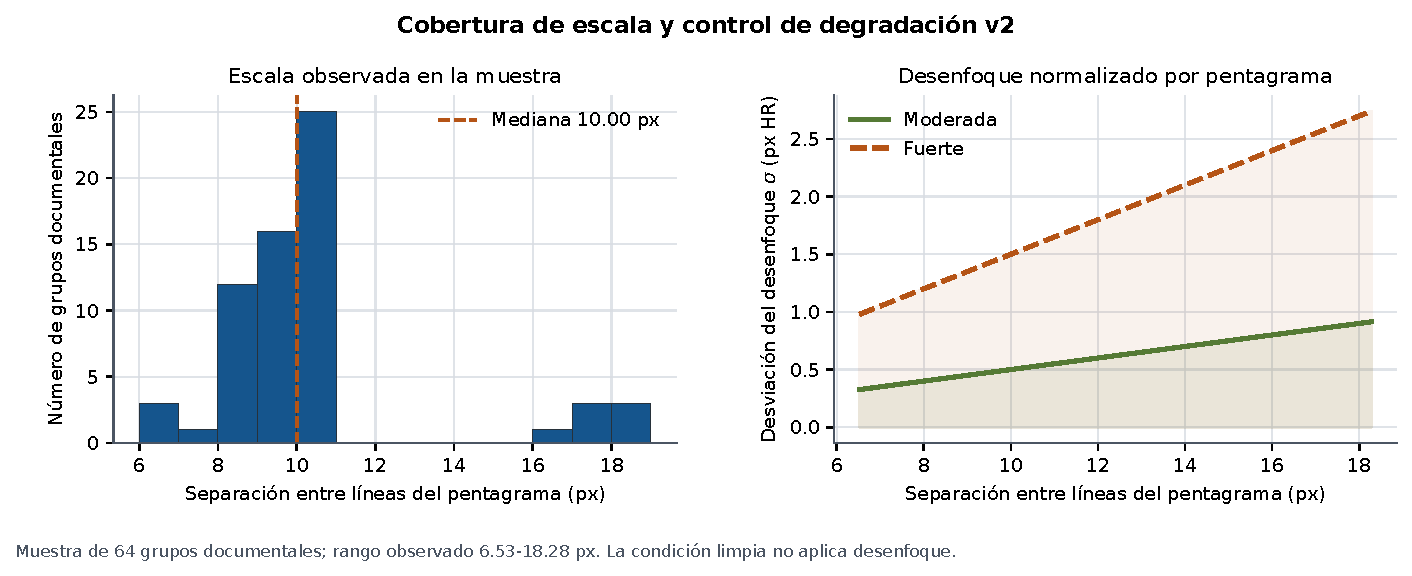
\includegraphics[width=\textwidth]{figures/context/staff-scale-and-blur.pdf}
  \caption[Escala de pentagrama y desenfoque en la muestra v2]{Distribución de separación entre líneas y desenfoque resultante en la muestra v2.
  Fuente: elaboración propia a partir de los 64 grupos documentales seleccionados y del protocolo congelado.}
  \label{fig:staff-scale}
\end{figure}

\chapter{Métodos y protocolo de evaluación}

\section{Métodos de referencia y modelos preentrenados}
\emph{Pendiente: selección, versiones, pesos, licencias, entradas y salidas.}

\section{Adaptación al dominio}
\emph{Pendiente: documentar la decisión GO/NO-GO y, únicamente si procede, el ajuste fino.}

\section{Métricas y unidades de análisis}
\emph{Pendiente: definir PSNR, SSIM, recursos, agregación, incertidumbre y comparaciones.}

\section{Evaluación específica de notación musical}
\emph{Pendiente: taxonomía de fallos, muestreo cualitativo y conservación de casos negativos.}

\section{Reproducibilidad}
\emph{Pendiente: configuraciones, entornos local/Kaggle, manifiestos y trazabilidad de evidencias.}

\chapter{Resultados}

\section{Resultados cuantitativos}
La Figura~\ref{fig:fidelity-means} muestra las medias por condición. Tanto EDSR como SwinIR
superaron a la interpolación bicúbica en PSNR-Y y SSIM-Y en las seis condiciones; los 24 intervalos
correspondientes ---dos métodos aprendidos, dos métricas y seis condiciones--- quedaron por encima
de cero. La magnitud, sin embargo, dependió claramente de la degradación. En \texttt{x2-clean},
EDSR mejoró a bicúbica en 4,345 dB y 0,0595 SSIM, mientras que SwinIR alcanzó 5,670 dB y 0,0695.
En \texttt{x2-strong} las ventajas se redujeron a 0,199 dB y 0,0074 para EDSR, y 0,176 dB y
0,0043 para SwinIR. Que los intervalos excluyan cero no convierte estos últimos efectos en una
mejora profesional relevante.

\begin{figure}[htbp]
  \centering
  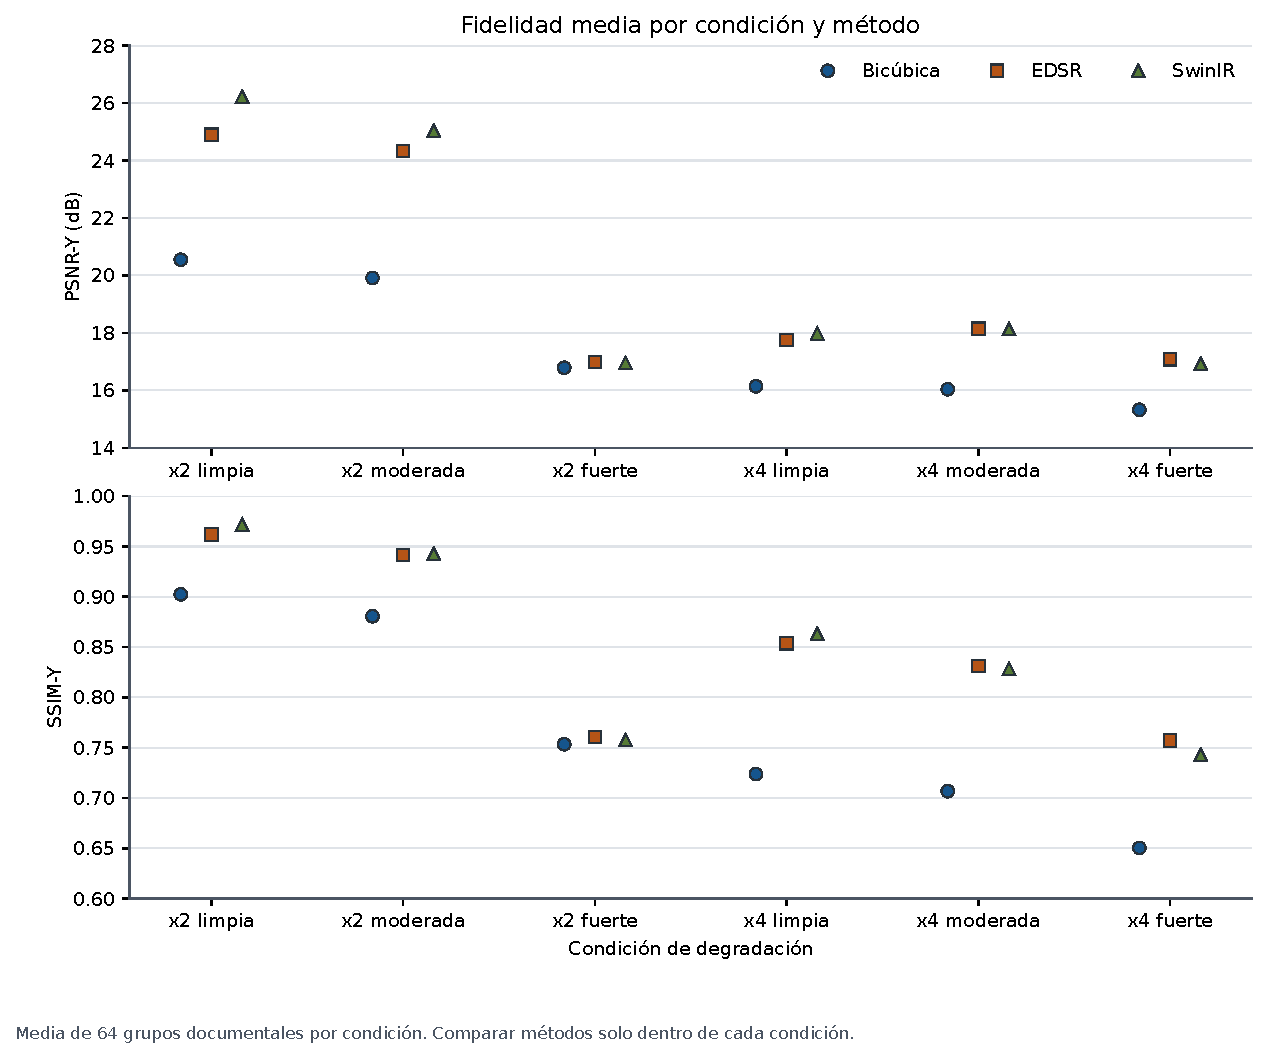
\includegraphics[width=\textwidth]{figures/results/fidelity-means.pdf}
  \caption{PSNR-Y y SSIM-Y medios para los 64 grupos documentales en cada condición. Las
  comparaciones solo son válidas dentro de la misma escala y perfil. Fuente: elaboración propia a
  partir del experimento SMB v2.}
  \label{fig:fidelity-means}
\end{figure}

La comparación directa entre las dos redes evita declarar un ganador por sus medias aisladas
(Tabla~\ref{tab:swinir-edsr}). Los intervalos favorecieron a SwinIR en las dos métricas para
\texttt{x2-clean}, \texttt{x2-moderate} y \texttt{x4-clean}. En \texttt{x2-strong} y
\texttt{x4-moderate}, el intervalo de PSNR cruzó cero y SSIM favoreció a EDSR. En
\texttt{x4-strong}, EDSR fue superior en ambas medidas. Por tanto, la mayor complejidad del
transformador no produjo una ventaja general.

\begin{table}[htbp]
  \centering
  \small
  \caption{Diferencia media emparejada SwinIR menos EDSR e intervalo percentil del 95\,\% por
  fuente. Un intervalo que cruza cero se marca como no resuelto. Fuente: elaboración propia.}
  \label{tab:swinir-edsr}
  \begin{tabular}{lrr}
    \toprule
    Condición & \(\Delta\) PSNR-Y (dB) & \(\Delta\) SSIM-Y \\
    \midrule
    x2 limpia    &  1,325 [1,178; 1,480]  &  0,0100 [0,0092; 0,0109] \\
    x2 moderada  &  0,704 [0,574; 0,835]  &  0,0014 [0,0002; 0,0024] \\
    x2 fuerte    & -0,023 [-0,074; 0,020] & -0,0031 [-0,0050; -0,0015] \\
    x4 limpia    &  0,230 [0,137; 0,336]  &  0,0094 [0,0074; 0,0116] \\
    x4 moderada  & -0,011 [-0,054; 0,033] & -0,0029 [-0,0042; -0,0015] \\
    x4 fuerte    & -0,152 [-0,197; -0,107]& -0,0142 [-0,0165; -0,0117] \\
    \bottomrule
  \end{tabular}
\end{table}

La Figura~\ref{fig:paired-deltas} completa esta lectura mostrando las ganancias de cada red frente
a la referencia bicúbica con su incertidumbre emparejada. Los resultados negativos y las
comparaciones no resueltas se conservaron en el análisis y no se sustituyeron por una selección de
condiciones favorables.

\begin{figure}[htbp]
  \centering
  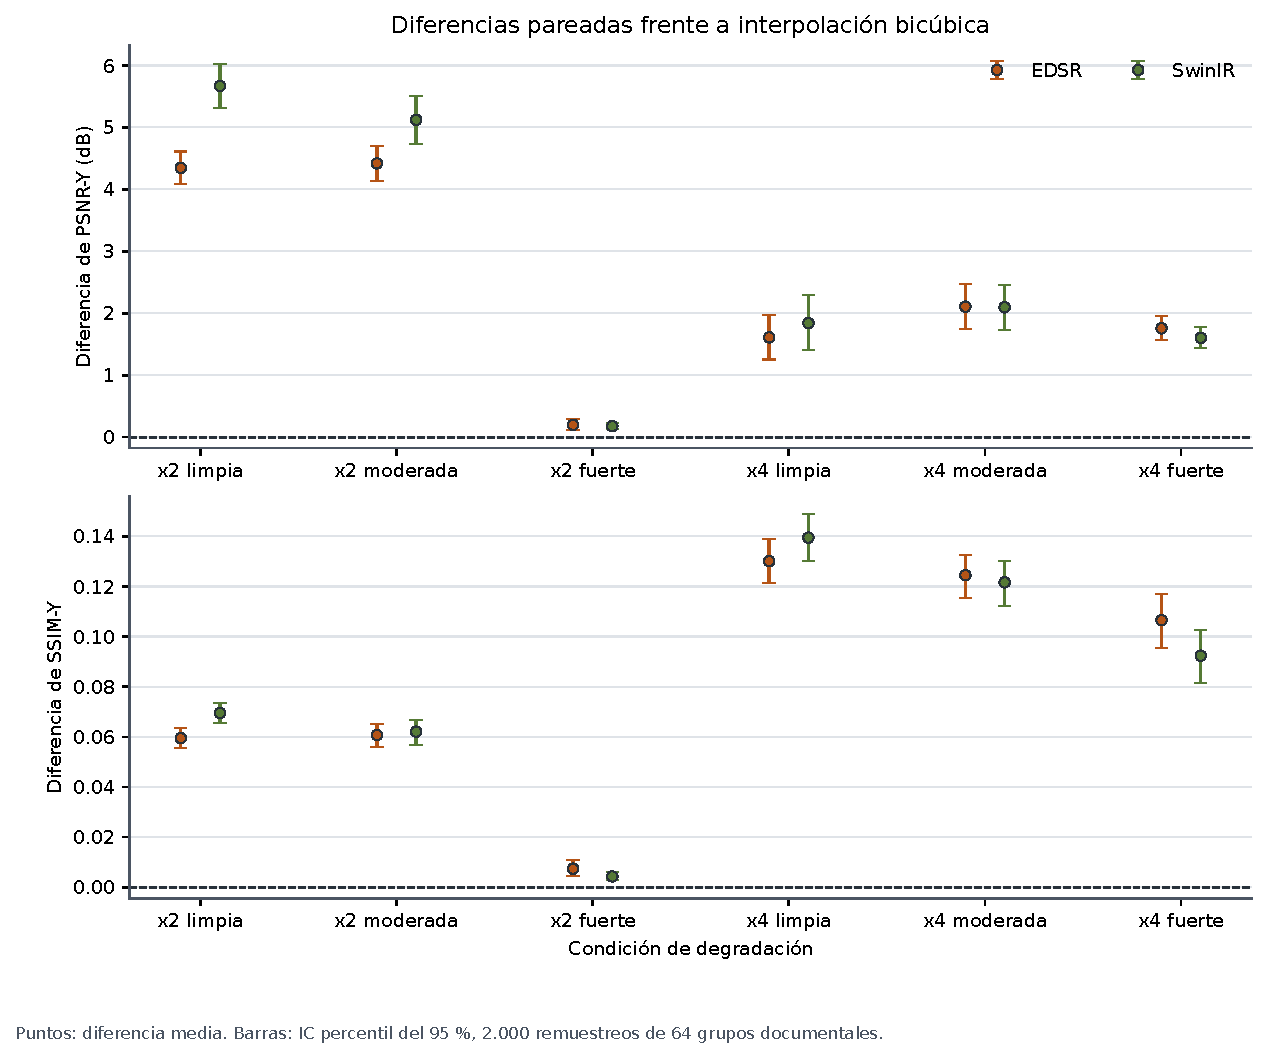
\includegraphics[width=\textwidth]{figures/results/paired-deltas-vs-bicubic.pdf}
  \caption{Ganancia media emparejada de EDSR y SwinIR respecto a bicúbica, con intervalos del
  95\,\% obtenidos al remuestrear las 64 fuentes. Fuente: elaboración propia.}
  \label{fig:paired-deltas}
\end{figure}

\section{Resultados cualitativos y fallos musicales}
La lectura visual sigue la secuencia referencia HR, entrada LR y salidas de los modelos.
La página completa permite comprobar disposición y legibilidad globales; las ampliaciones
muestran separaciones, contornos y signos que se pierden al reducir la página para imprimirla.
En cada comparación se utiliza exactamente la misma región y el mismo tamaño de visualización.
Cada caso de detalle ocupa una página propia, con dos columnas, para que los símbolos se puedan
examinar a mayor tamaño. Las imágenes se incrustan en PDF a su resolución nativa, sin reducción
previa de píxeles ni compresión con pérdidas. Las vistas de página completa aportan contexto;
el juicio sobre trazos finos se apoya en las ampliaciones y en el zoom del documento digital.
La LR se amplía por vecino más próximo, sin suavizado añadido. Los casos pertenecen a la revisión
cualitativa fijada; los recortes se eligieron después para explicar sus observaciones, no para
recalcular valoraciones ni para estimar la frecuencia de un defecto.

En las 18 valoraciones fijas se registró \emph{sin incidencia clara} en cuatro de los seis casos
bicúbicos y en dos de los seis casos de cada red. Se observaron incidencias en dos casos bicúbicos,
cuatro EDSR y cuatro SwinIR. Estos recuentos describen únicamente las seis páginas fijadas y no son
tasas de error ni permiten ordenar métodos por seguridad.

Los tres métodos quedaron sin incidencias claras en las condiciones x2 limpia y x2 moderada. En el
caso x2 fuerte, la entrada seguía siendo legible y bicúbica no
añadió un defecto claro, pero tampoco produjo una mejora apreciable; EDSR y SwinIR perdieron detalle
en símbolos y añadieron textura o \emph{ringing}. En los casos \(\times 4\) aparecieron
simplificación de símbolos, corrupción de texto o dígitos y reconstrucción de líneas rectas como
trazos ligeramente curvos. En \texttt{x4-moderate}, SwinIR reconstruyó visualmente las notas mejor
que EDSR en el caso revisado, pese a mantener defectos en otros símbolos o dígitos. En x4 fuerte,
parte del daño procedía ya de la degradación y ninguno de los tres métodos lo
recuperó de manera fiable.

La Figura~\ref{fig:pretrained-qualitative} hace visible esa discrepancia entre una puntuación
global y la lectura localizada. En el caso fijo \texttt{smb-test-000210}, EDSR y SwinIR obtuvieron
valores prácticamente empatados ---18,314 y 18,311 dB de PSNR-Y; 0,7960 y 0,7932 de SSIM-Y---,
por encima de la bicúbica ---15,949 dB y 0,6696---. Sin embargo, el recorte revela que la valoración
no depende solo de nitidez: las redes recuperan mejor las notas que la interpolación, pero alteran
textura, dígitos y geometría fina; en esta región, el revisor consideró más reconocibles las notas
de SwinIR que las de EDSR. La referencia HR impide confundir una salida más contrastada con una
reconstrucción necesariamente correcta.

\begin{figure}[htbp]
  \centering
  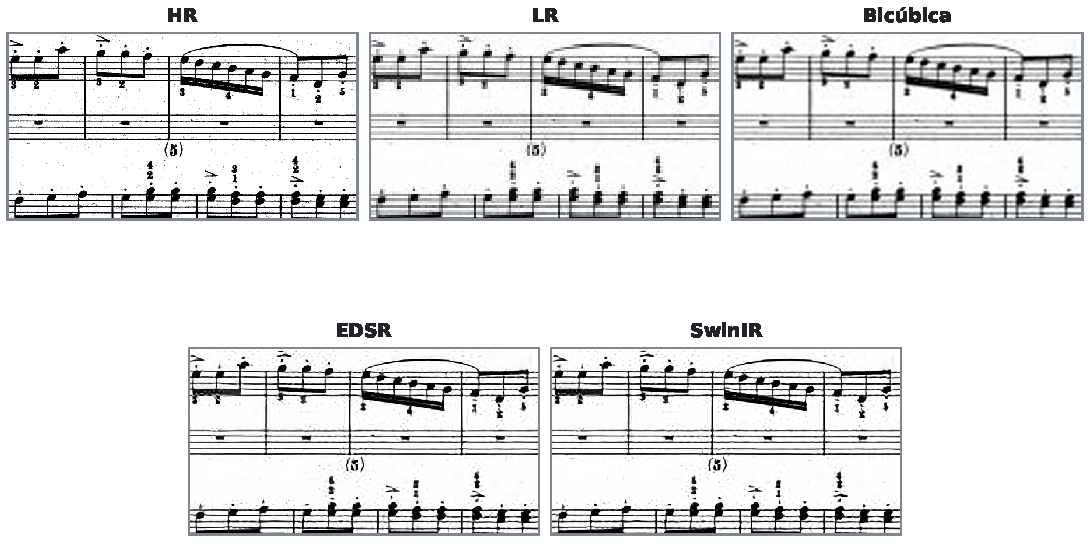
\includegraphics[width=\textwidth]{figures/results/pretrained-comparison-x4-moderate.pdf}
  \caption[Comparación cualitativa de los métodos preentrenados]{Referencia, entrada LR y salidas
  de los tres comparadores para el caso fijo \texttt{smb-test-000210} bajo
  \texttt{x4-moderate}. La LR se amplía por vecino más próximo. El ejemplo conserva tanto la
  mejora sobre bicúbica como los defectos que impiden declarar un ganador solo por PSNR-Y o
  SSIM-Y. Fragmento de la Sonata L.55/K.330 de Domenico Scarlatti, identificada como
  \texttt{scarlatti\_l055k330}. Fuente: elaboración propia a partir de SMB
  \cite{smbDatasetCard}.}
  \label{fig:pretrained-qualitative}
\end{figure}

La Figura~\ref{fig:pretrained-details} reúne tres situaciones distintas del muestreo fijo.
En A, la entrada x2 limpia conserva la estructura y las redes definen los trazos sin una incidencia
clara en la revisión. En B, la notación de la referencia sigue siendo reconocible en LR, pero las
salidas aprendidas modifican los contornos y la textura: conviene observar el fondo alrededor de
las notas y las pequeñas separaciones, además del contraste. En C, x4 fuerte ya ha difuminado
trazos finos y texto; la salida puede parecer más perfilada sin recuperar su forma original.
Los tres casos corresponden a grupos documentales diferentes y sirven para ilustrar comportamientos heterogéneos;
la comparación controlada de severidad sobre un mismo fragmento está en la
Figura~\ref{fig:degradation-profiles}.

\begin{figure}[p]
  \centering
  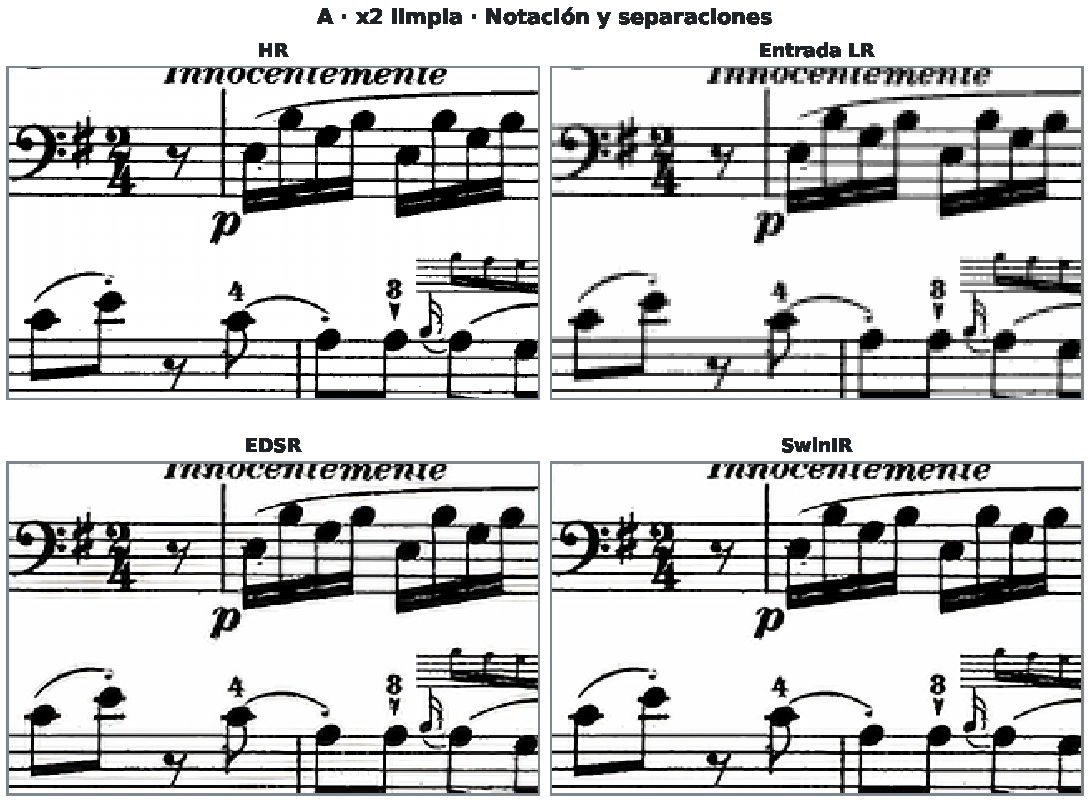
\includegraphics[page=1,width=\textwidth]{figures/results/pretrained-detail-gallery.pdf}
  \caption[Detalle de reconstrucciones favorables y artefactos preentrenados]{Ampliaciones
  emparejadas de tres casos SMB de la revisión fija, en tres láminas consecutivas. En esta primera
  lámina, A: \texttt{smb-test-000252}, x2 limpia,
  \texttt{haydn\_sonata53\_3}, de Joseph Haydn. B: \texttt{smb-test-000264}, x2 fuerte,
  \texttt{hummel\_prelude67\_04}, de Johann Nepomuk Hummel. C: \texttt{smb-test-000526}, x4 fuerte,
  \texttt{mozart\_sonata03\_2}, de Wolfgang Amadeus Mozart. La cercanía a HR debe juzgarse en los
  contornos, espacios y marcas pequeñas; una salida más nítida puede conservar o añadir defectos.
  Fuente: elaboración propia a partir de SMB \cite{smbDatasetCard}; coordenadas idénticas para
  todos los paneles de cada caso, sin realce adicional.}
  \label{fig:pretrained-details}
\end{figure}
\clearpage

\begin{figure}[p]
  \centering
  \includegraphics[page=2,width=\textwidth]{figures/results/pretrained-detail-gallery.pdf}
  \caption[B: x2 fuerte, Hummel]{Textura y contornos de HR, LR, EDSR y SwinIR en el caso fijo Hummel, ya identificado en la Figura~\ref{fig:pretrained-details}. Se conserva el mismo encuadre sin remuestrear los píxeles de las salidas. Fuente: SMB \cite{smbDatasetCard}.}
\end{figure}
\clearpage

\begin{figure}[p]
  \centering
  \includegraphics[page=3,width=\textwidth]{figures/results/pretrained-detail-gallery.pdf}
  \caption[C: x4 fuerte, Mozart]{Pérdida de trazos y texto en el caso fijo Mozart, identificado en la Figura~\ref{fig:pretrained-details}. La reconstrucción puede perfilar el trazo sin recuperar su geometría original. Fuente: SMB \cite{smbDatasetCard}.}
\end{figure}
\clearpage


La Tabla~\ref{tab:qualitative-origin} separa el origen observable del problema. \emph{No claro} no
significa que la salida sea perfecta, sino que no se identificó un defecto atribuible al método en
el caso. \emph{Introducido/amplificado} indica una diferencia problemática respecto de LR, mientras
que \emph{no recuperado} indica que el daño ya estaba presente en LR. La tabla evita sumar ambos
fenómenos como si fueran equivalentes.

\begin{table}[htbp]
  \centering
  \footnotesize
  \setlength{\tabcolsep}{3pt}
  \caption{Origen observable de las incidencias en los seis casos cualitativos fijos. Fuente:
  elaboración propia a partir de la revisión del estudiante.}
  \label{tab:qualitative-origin}
  \begin{tabular}{p{0.15\textwidth}p{0.24\textwidth}p{0.25\textwidth}p{0.25\textwidth}}
    \toprule
    Condición & Bicúbica & EDSR & SwinIR \\
    \midrule
    x2 limpia & No claro & No claro & No claro \\
    x2 moderada & No claro & No claro & No claro \\
    x2 fuerte & No claro; sin mejora apreciable & Introducido o amplificado & Introducido o amplificado \\
    x4 limpia & No claro; sin mejora apreciable & Introducido o amplificado & Introducido o amplificado \\
    x4 moderada & Introducido o amplificado & Introducido o amplificado & Introducido o amplificado \\
    x4 fuerte & Presente en LR y no recuperado & Introducido o amplificado sobre LR dañada & Introducido o amplificado sobre LR dañada \\
    \bottomrule
  \end{tabular}
\end{table}

No se marcó ningún \emph{cambio musicalmente plausible} como categoría separada, pero sí símbolos
alterados o perdidos en cuatro casos EDSR y tres SwinIR. Por ello, la ausencia de aquella etiqueta
no demuestra conservación semántica. La evidencia cualitativa contradice cualquier interpretación
según la cual una mejora promedio de PSNR o SSIM garantice que todos los elementos musicales se
reconstruyan correctamente.

Estos datos no permiten estimar sensibilidad, especificidad ni tasa de errores. La selección
determinista cubre condiciones, no tipos de símbolo, compositores, tipografías o severidades reales;
además, la revisión fue realizada por un único evaluador no ciego. Su fuerza reside en refutar una
interpretación demasiado amplia de las métricas y en documentar modos de fallo concretos, no en
probar que un método sea más seguro que otro en toda la población.

\clearpage
\section{Adaptación secundaria de EDSR}
La selección por validación produjo el punto de control del paso 1.500 para x2, con L1 RGB media
0,01409, y el del paso 2.500 para x4, con 0,03158. La Figura~\ref{fig:adaptation-checkpoints}
muestra que x2 dejó de mejorar de forma sostenida, mientras que x4 alcanzó su mínimo en el último
punto permitido. Por tanto, el resultado x4 describe el presupuesto congelado y podría subestimar
una mejora posterior; no se prolongó el entrenamiento después de observar la prueba.

\begin{figure}[htbp]
  \centering
  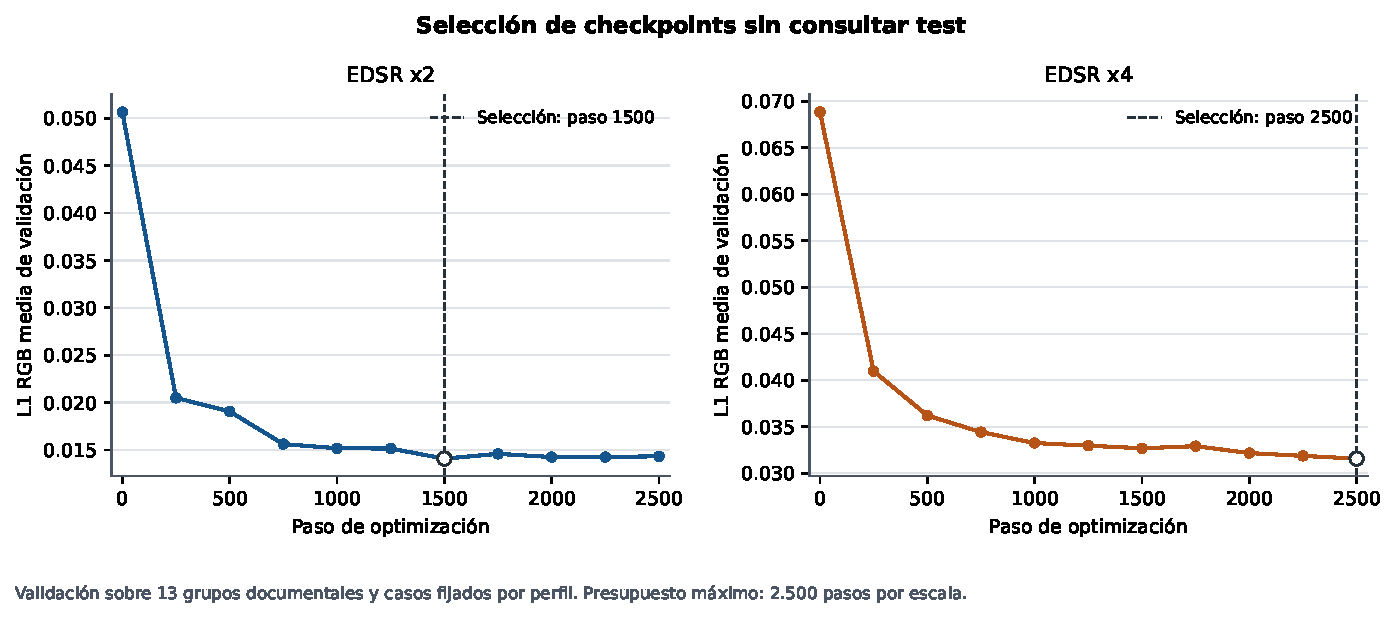
\includegraphics[width=\textwidth]{figures/results/adaptation-checkpoint-selection.pdf}
  \caption{Pérdida L1 RGB de validación y puntos de control elegidos para EDSR x2 y x4. La
  selección utiliza 13 grupos documentales y no consulta los 20 grupos documentales de prueba. Fuente:
  elaboración propia a partir del estudio de adaptación.}
  \label{fig:adaptation-checkpoints}
\end{figure}

El EDSR adaptado superó al EDSR oficial en PSNR-Y y SSIM-Y para las seis condiciones. Los doce
intervalos emparejados del 95\,\% quedaron por encima de cero. La ganancia PSNR-Y abarcó de
3,242 dB en x4 moderada a 7,844 dB en x2 fuerte; la ganancia SSIM-Y, de 0,0169 en x2 limpia a
0,1949 en x2 fuerte. En x2 mejoraron los 20 grupos documentales en ambas métricas. En x4, SSIM-Y mejoró en los
20; PSNR-Y lo hizo en 20 grupos bajo degradación limpia, 19 bajo moderada y 18 bajo fuerte.

\begin{table}[htbp]
  \centering
  \footnotesize
  \caption{Diferencia media emparejada EDSR adaptado menos EDSR oficial, con intervalo percentil
  del 95\,\% sobre 20 grupos documentales de prueba. Fuente: elaboración propia.}
  \label{tab:adaptation-deltas}
  \begin{tabular}{lrr}
    \toprule
    Condición & \(\Delta\) PSNR-Y (dB) & \(\Delta\) SSIM-Y \\
    \midrule
    x2 limpia   & 3,955 [3,492; 4,373] & 0,0169 [0,0143; 0,0200] \\
    x2 moderada & 4,719 [4,106; 5,336] & 0,0387 [0,0361; 0,0415] \\
    x2 fuerte   & 7,844 [7,328; 8,292] & 0,1949 [0,1786; 0,2104] \\
    x4 limpia   & 3,599 [2,978; 4,186] & 0,0602 [0,0487; 0,0722] \\
    x4 moderada & 3,242 [2,647; 3,771] & 0,0796 [0,0660; 0,0933] \\
    x4 fuerte   & 3,703 [2,723; 4,690] & 0,1558 [0,1365; 0,1746] \\
    \bottomrule
  \end{tabular}
\end{table}

La Figura~\ref{fig:adaptation-deltas} permite comparar magnitudes y denominadores sin mezclar este
estudio con los 64 grupos documentales del experimento principal. El modelo adaptado también superó a bicúbica
en ambas métricas y condiciones al nivel agregado. Sin embargo, las dos fuentes que empeoraron en
PSNR-Y frente al EDSR oficial bajo x4 fuerte fueron también las de menor separación de pentagrama
de la prueba. Es una observación \emph{post hoc} de solo dos casos, útil como hipótesis y no como
conclusión de subgrupo.
Los valores completos y sus intervalos se recogen en la Tabla~\ref{tab:adaptation-deltas}.

\begin{figure}[htbp]
  \centering
  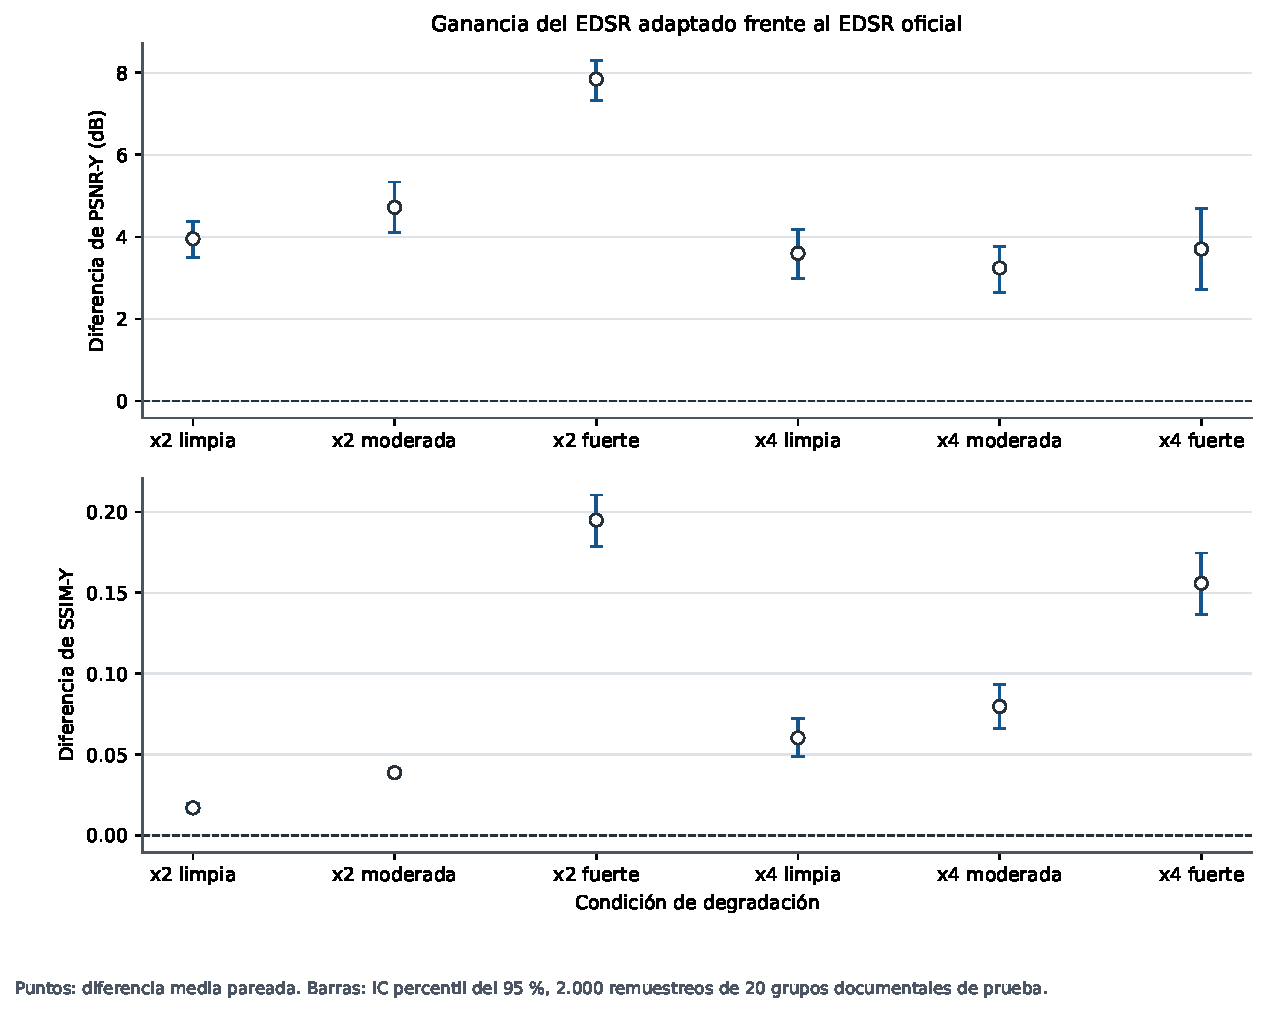
\includegraphics[width=0.92\textwidth]{figures/results/adaptation-deltas-vs-pretrained.pdf}
  \caption{Ganancia del EDSR adaptado respecto del EDSR oficial en 20 grupos documentales de prueba, con
  intervalos emparejados del 95\,\%. Fuente: elaboración propia a partir del estudio secundario.}
  \label{fig:adaptation-deltas}
\end{figure}

La revisión del estudiante clasificó los casos x2/x4 limpios y moderados como mejora sin defecto
nuevo claro, y los dos casos fuertes como daño ya presente en LR y no recuperado. Ninguno de los
seis se clasificó como daño introducido o amplificado por el EDSR adaptado. En los cuatro primeros,
el ajuste redujo halos y textura y definió mejor pentagramas y notación; persistieron limitaciones
menores en texto y en cabezas de nota muy próximas. En x2 fuerte, el mayor contraste no recuperó
alteraciones, ornamentos, líneas adicionales, texto ni dígitos pequeños. En x4 fuerte, el resultado
fue más legible que el EDSR oficial y reconstruyó mejor cabezas rellenas, plicas y ligaduras, pero
no recuperó digitaciones, símbolos pequeños, blancas ni texto. Podría servir para una consulta
aproximada, no para una interpretación musical final.

Las Figuras~\ref{fig:adapted-full-page}, \ref{fig:adapted-moderate}
y~\ref{fig:adapted-strong} muestran ambas caras del resultado con casos fijados antes de la
revisión. La primera conserva la página completa: permite verificar que el procesamiento mantiene
la disposición, los cinco sistemas, los márgenes y la densidad global, y muestra que el EDSR
adaptado se aproxima a la referencia con trazos más definidos que el oficial. Esta vista, sin
embargo, hace pequeños los detalles donde se decide la fidelidad musical; por eso se acompaña del
recorte alineado de la Figura~\ref{fig:adapted-moderate}. En \texttt{x4-moderate}, el ejemplo
\texttt{smb-test-000451} pasó de 23,184 a 26,684 dB de PSNR-Y y de 0,9254 a 0,9749 de SSIM-Y
entre el EDSR oficial y el adaptado. El recorte permite relacionar esa ganancia con menos halo,
trazos más rectos y una geometría más próxima a HR, sobre todo en pentagramas, ligaduras y
alteraciones. No equivale a afirmar que el modelo mejore todos los símbolos de la página.

\begin{figure}[p]
  \centering
  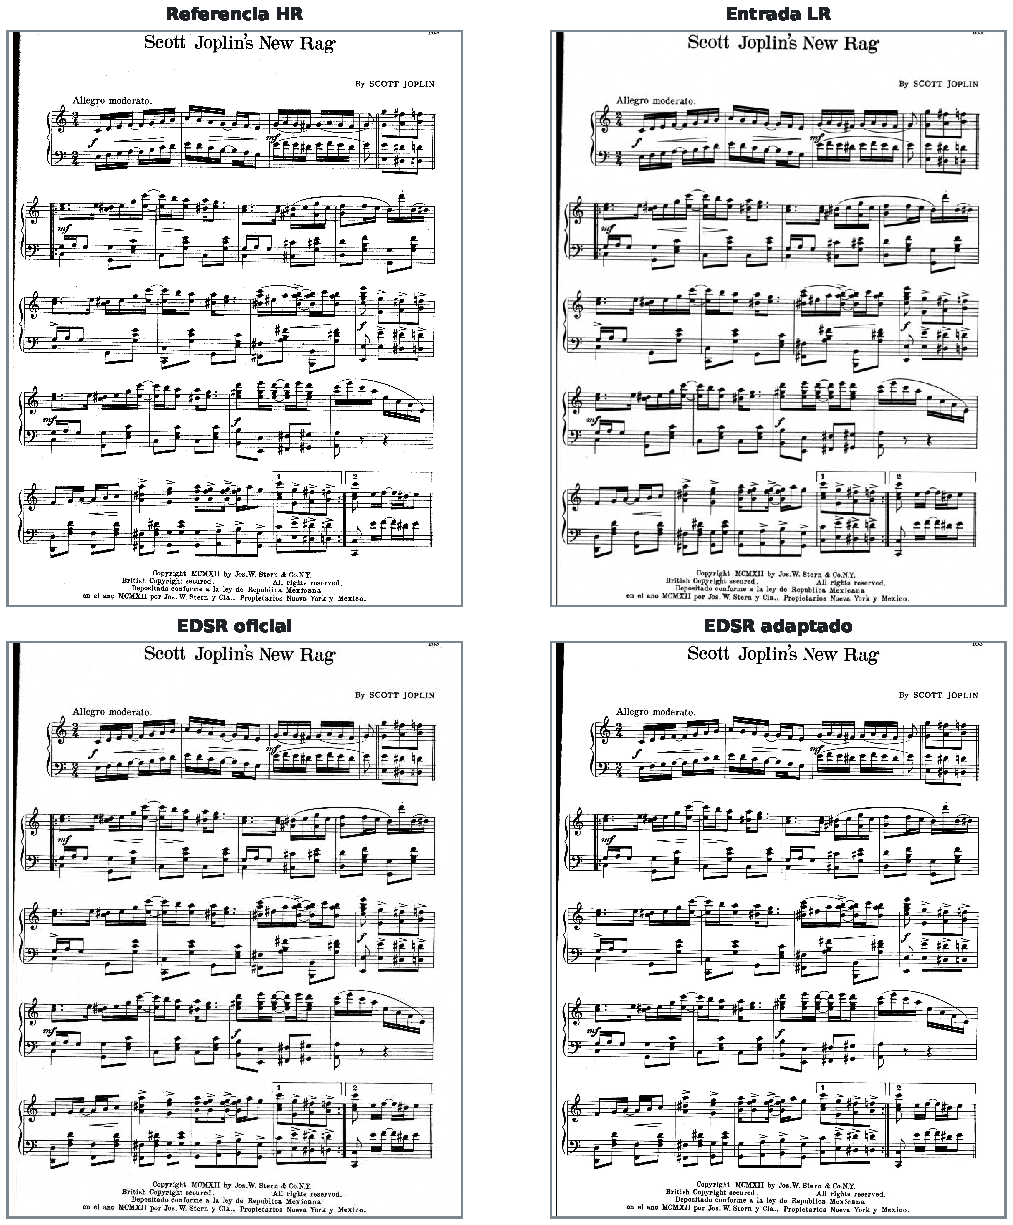
\includegraphics[width=\textwidth,height=0.82\textheight,keepaspectratio]{figures/results/adapted-full-page-x4-moderate.pdf}
  \caption[Comparación de página completa tras adaptar EDSR]{Comparación de página completa del
  caso fijo \texttt{smb-test-000451} bajo \texttt{x4-moderate}. La vista completa permite valorar
  estructura y legibilidad globales; los detalles se inspeccionan en la
  Figura~\ref{fig:adapted-moderate}. La LR está ampliada por vecino más próximo. Página de
  \emph{Scott Joplin's New Rag}, de Scott Joplin. Fuente: elaboración propia a partir de SMB,
  distribuido como CC BY-NC 4.0 \cite{smbDatasetCard,ccByNc40}; LR y reconstrucciones son
  transformaciones realizadas para este TFG.}
  \label{fig:adapted-full-page}
\end{figure}

\begin{figure}[htbp]
  \centering
  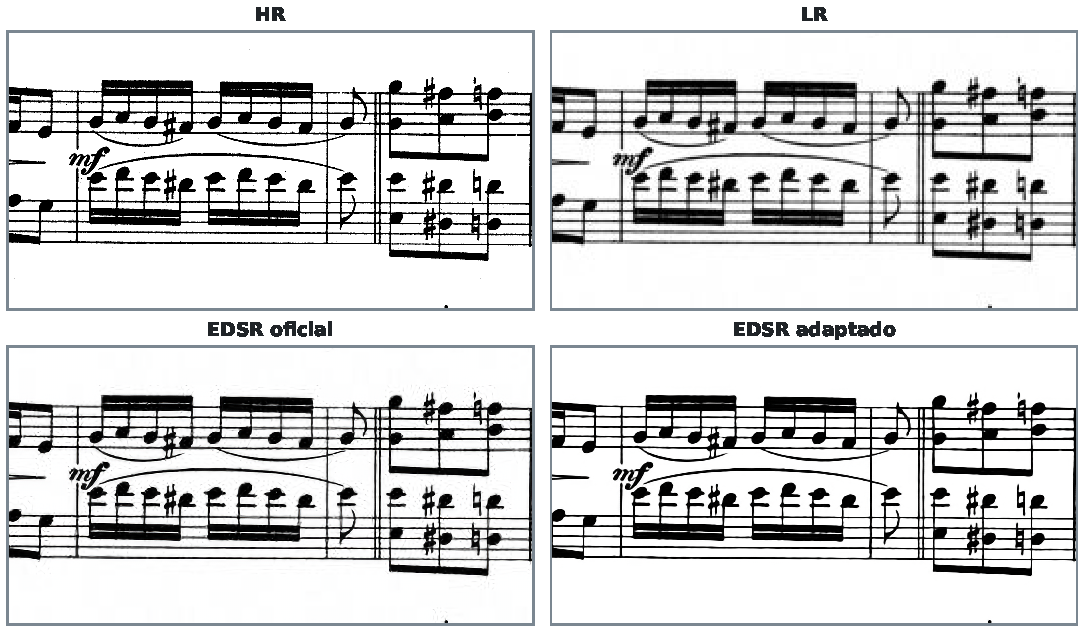
\includegraphics[width=\textwidth]{figures/results/adapted-comparison-x4-moderate.pdf}
  \caption[Mejora cualitativa del EDSR adaptado en x4 moderada]{Entrada y reconstrucciones del caso
  fijo \texttt{smb-test-000451} bajo degradación \texttt{x4-moderate}. La LR se amplía por vecino
  más próximo para visualizarla al tamaño HR. El EDSR adaptado reduce la textura y los halos del
  modelo oficial y aproxima mejor los trazos de la referencia. Fragmento de
  \emph{Scott Joplin's New Rag}, de Scott Joplin. Fuente: elaboración propia a partir de SMB
  \cite{smbDatasetCard}.}
  \label{fig:adapted-moderate}
\end{figure}

El caso \texttt{smb-test-000655}, en cambio, demuestra por qué una mejora métrica no autoriza una
promesa de restauración. Bajo \texttt{x4-strong}, el EDSR adaptado elevó PSNR-Y de 17,400 a
20,104 dB y SSIM-Y de 0,7860 a 0,9205 respecto del oficial, y eliminó gran parte de su textura
espuria. Aun así, la LR ya había perdido digitaciones, detalles internos y texto que el modelo no
podía deducir con fidelidad. En la Figura~\ref{fig:adapted-strong} el resultado adaptado es más
limpio, pero no es equivalente a la referencia ni apto para una edición musical final.

\begin{figure}[htbp]
  \centering
  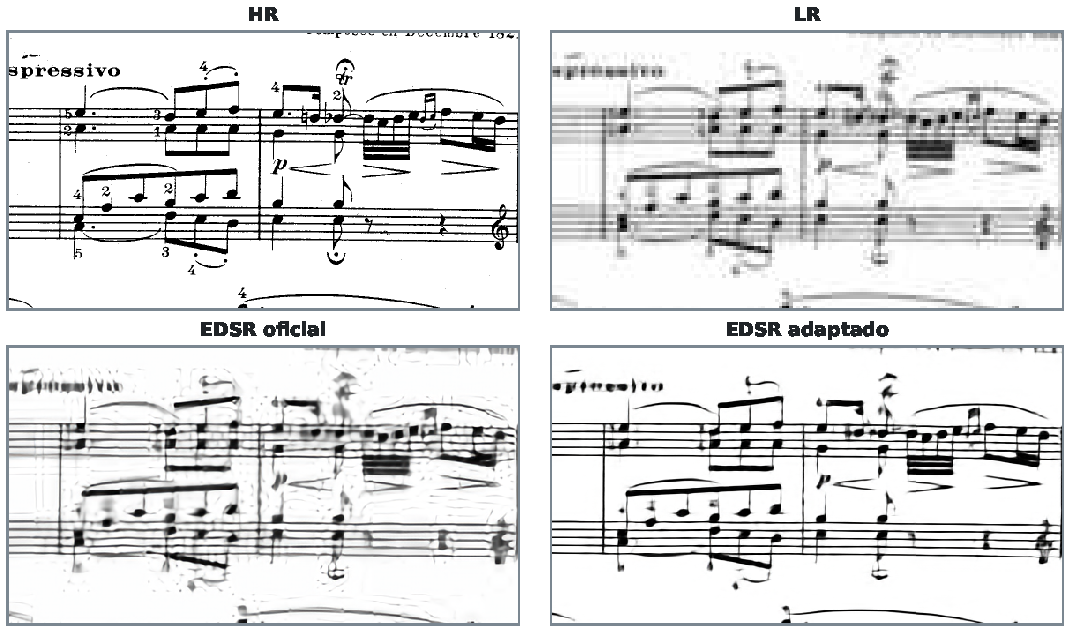
\includegraphics[width=\textwidth]{figures/results/adapted-limit-x4-strong.pdf}
  \caption[Límite del EDSR adaptado en x4 fuerte]{Caso fijo \texttt{smb-test-000655} bajo
  degradación \texttt{x4-strong}. La adaptación reduce los artefactos del EDSR oficial, pero no
  recupera toda la información ausente en LR; destacan la digitación y los signos pequeños. La LR
  se muestra ampliada por vecino más próximo. Fragmento de la Sonata para piano n.º 31, op.~110,
  de Ludwig van Beethoven, identificada como \texttt{beethoven\_sonata31\_1}. Fuente: elaboración
  propia a partir de SMB \cite{smbDatasetCard}.}
  \label{fig:adapted-strong}
\end{figure}

La Figura~\ref{fig:adapted-details} acerca ambos casos a detalles de tamaño comparable en el papel.
En A se pueden seguir las líneas y los límites de las alteraciones desde HR hasta el modelo
adaptado: la mejora consiste en aproximar la geometría de referencia, además de limpiar el fondo.
En B, las digitaciones y las marcas pequeñas permiten comprobar el límite: definir una mancha no
implica reconstruir el signo que ocupaba esa posición. Esta comparación ayuda a distinguir la
reducción de artefactos del EDSR oficial de la recuperación efectiva de información musical.

\begin{figure}[p]
  \centering
  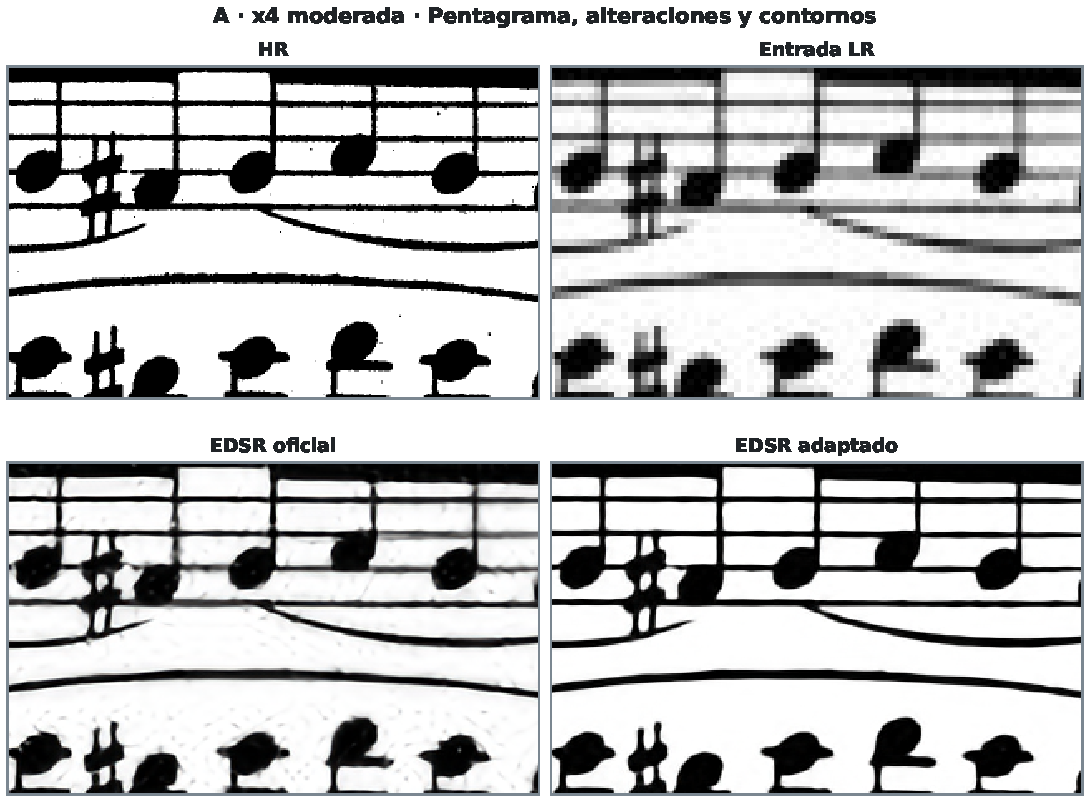
\includegraphics[page=1,width=\textwidth]{figures/results/adapted-detail-gallery.pdf}
  \caption[Detalle de la mejora y del límite del ajuste fino]{Las mismas regiones antes y después
  de adaptar EDSR, en dos láminas consecutivas. En esta primera, A, \emph{Scott Joplin's New Rag}, de Scott Joplin, caso
  \texttt{smb-test-000451} en x4 moderada; B, Sonata para piano n.º 31, op.~110, de Ludwig van
  Beethoven, caso \texttt{smb-test-000655} en x4 fuerte, en la siguiente lámina. El primer caso muestra la aproximación
  de los trazos a HR; el segundo conserva pérdidas visibles en elementos pequeños. Fuente:
  elaboración propia a partir de SMB \cite{smbDatasetCard}. Cada caso muestra el mismo recorte
  en HR, LR y ambas reconstrucciones, sin retoques de contraste ni limpieza posterior.}
  \label{fig:adapted-details}
\end{figure}
\clearpage

\begin{figure}[p]
  \centering
  \includegraphics[page=2,width=\textwidth]{figures/results/adapted-detail-gallery.pdf}
  \caption[B: límite de la adaptación, Beethoven]{Ampliación del caso Beethoven x4 fuerte, identificado en la Figura~\ref{fig:adapted-details}. El adaptado reduce artefactos, pero las digitaciones y marcas pequeñas de HR siguen sin reconstruirse con fidelidad. Fuente: SMB \cite{smbDatasetCard}.}
\end{figure}
\clearpage


Estos seis casos detectan límites, pero no permiten estimar su frecuencia ni demuestran corrección
semántica. En consecuencia, la adaptación respalda una mejora de fidelidad dentro de SMB y
degradaciones coincidentes, no una restauración musical autónoma.

\clearpage
\section{Transferencia externa y demostrador}
Al aplicar el EDSR adaptado sin reajuste a las doce obras externas, la diferencia media respecto al
EDSR oficial fue positiva en PSNR-Y y SSIM-Y en las seis condiciones
(Tabla~\ref{tab:external-deltas}). Los seis intervalos de PSNR-Y excluyeron cero; en SSIM-Y lo
hicieron cinco. La única comparación no resuelta fue x2 limpia, cuya media fue 0,0050 y cuyo
intervalo abarcó de -0,0014 a 0,0110. El resultado sostiene transferencia de fidelidad a otra
colección bajo el mismo generador sintético, sin demostrar recuperación de entradas LR naturales.

\begin{table}[htbp]
  \centering
  \footnotesize
  \caption{Diferencia media emparejada EDSR adaptado menos EDSR oficial en el corpus externo, con
  intervalo percentil del 95\,\% sobre doce obras. Fuente: elaboración propia.}
  \label{tab:external-deltas}
  \begin{tabular}{lrr}
    \toprule
    Condición & \(\Delta\) PSNR-Y (dB) & \(\Delta\) SSIM-Y \\
    \midrule
    x2 limpia   & 3,187 [1,193; 5,462] & 0,0050 [-0,0014; 0,0110] \\
    x2 moderada & 6,446 [5,299; 7,472] & 0,0287 [0,0248; 0,0340] \\
    x2 fuerte   & 8,204 [7,697; 8,724] & 0,1581 [0,1482; 0,1683] \\
    x4 limpia   & 2,440 [1,509; 3,418] & 0,0329 [0,0202; 0,0450] \\
    x4 moderada & 1,838 [0,990; 2,638] & 0,0433 [0,0319; 0,0553] \\
    x4 fuerte   & 2,376 [1,539; 3,242] & 0,0981 [0,0767; 0,1177] \\
    \bottomrule
  \end{tabular}
\end{table}

La revisión fija clasificó ocho casos como aceptables para consulta, tres como aceptables con
reservas y uno como rechazado. Los seis casos x2 fueron aceptados; en x4 limpia y moderada hubo un
aceptable y uno con reservas por condición; en x4 fuerte hubo uno con reservas y un rechazo. Este
último correspondió a una parte de percusión dispersa con cabezas y tipografía finas que no se
recuperaron de forma suficientemente consultable. En cinco casos no se observó defecto nuevo claro
y en siete el problema se atribuyó a información perdida en LR y no recuperada. Ninguno se marcó
como defecto introducido o amplificado, pero doce observaciones de un único revisor no demuestran
ausencia poblacional de ese riesgo.

\begin{figure}[htbp]
  \centering
  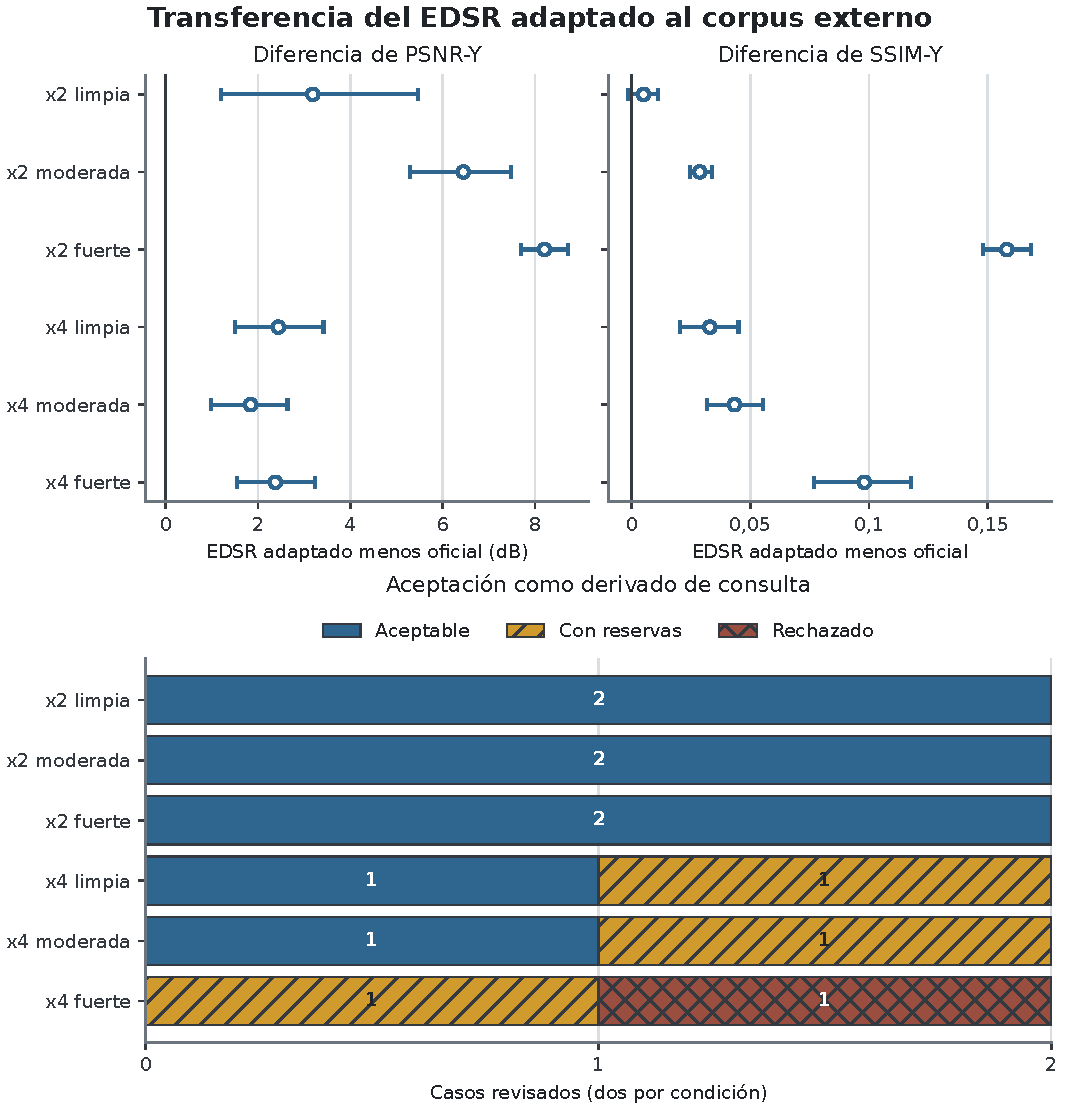
\includegraphics[width=0.98\textwidth]{figures/results/external-pilot-transfer.pdf}
  \caption[Transferencia y aceptación en el piloto externo]{Arriba, diferencia del EDSR adaptado
  respecto al oficial con intervalos emparejados del 95\,\% sobre doce obras externas. Abajo,
  decisiones del estudiante en los doce casos fijados, dos por condición. Los recuentos describen
  la muestra revisada y no son tasas de éxito. Fuente: elaboración propia.}
  \label{fig:external-pilot-transfer}
\end{figure}

La Figura~\ref{fig:external-pilot-transfer} muestra conjuntamente la transferencia cuantitativa y
las decisiones de consulta sin convertir estas últimas en una tasa poblacional. Las observaciones
convergieron en una limitación: el modelo adaptado redujo halos y textura y
definió mejor pentagramas y símbolos principales, pero el texto, los dígitos y la geometría fina
fueron los primeros elementos en no recuperarse al aumentar la degradación. En los dos escaneos HR
el revisor percibió incluso trazos más limpios, lo cual puede ser útil para consulta, pero no cambia
la condición del original como referencia documental ni prueba restauración histórica.

Las Figuras~\ref{fig:external-accepted} y~\ref{fig:external-rejected} hacen verificable esa síntesis
en el contexto completo de dos páginas que ya pertenecían al muestreo cualitativo fijo. No se
eligieron después por sus métricas: representan, respectivamente, un caso aceptado para consulta y
el único rechazo. Las otras diez comparaciones completas se reúnen en el
Anexo~\ref{app:external-case-atlas}; junto con estas dos, exponen visualmente las doce decisiones
sin omitir los casos con reservas. En \emph{Three Revelations from the Lotus Sutra}, la degradación x2 fuerte
difumina texto, alteraciones y trazos finos; el EDSR oficial mantiene un aspecto borroso, mientras
que el adaptado recupera contraste y continuidad suficientes para la consulta de la parte. No
reconstruye con exactitud todos los símbolos pequeños, por lo que la mejora visual no se traduce en
una garantía de identidad con HR.

\begin{figure}[p]
  \centering
  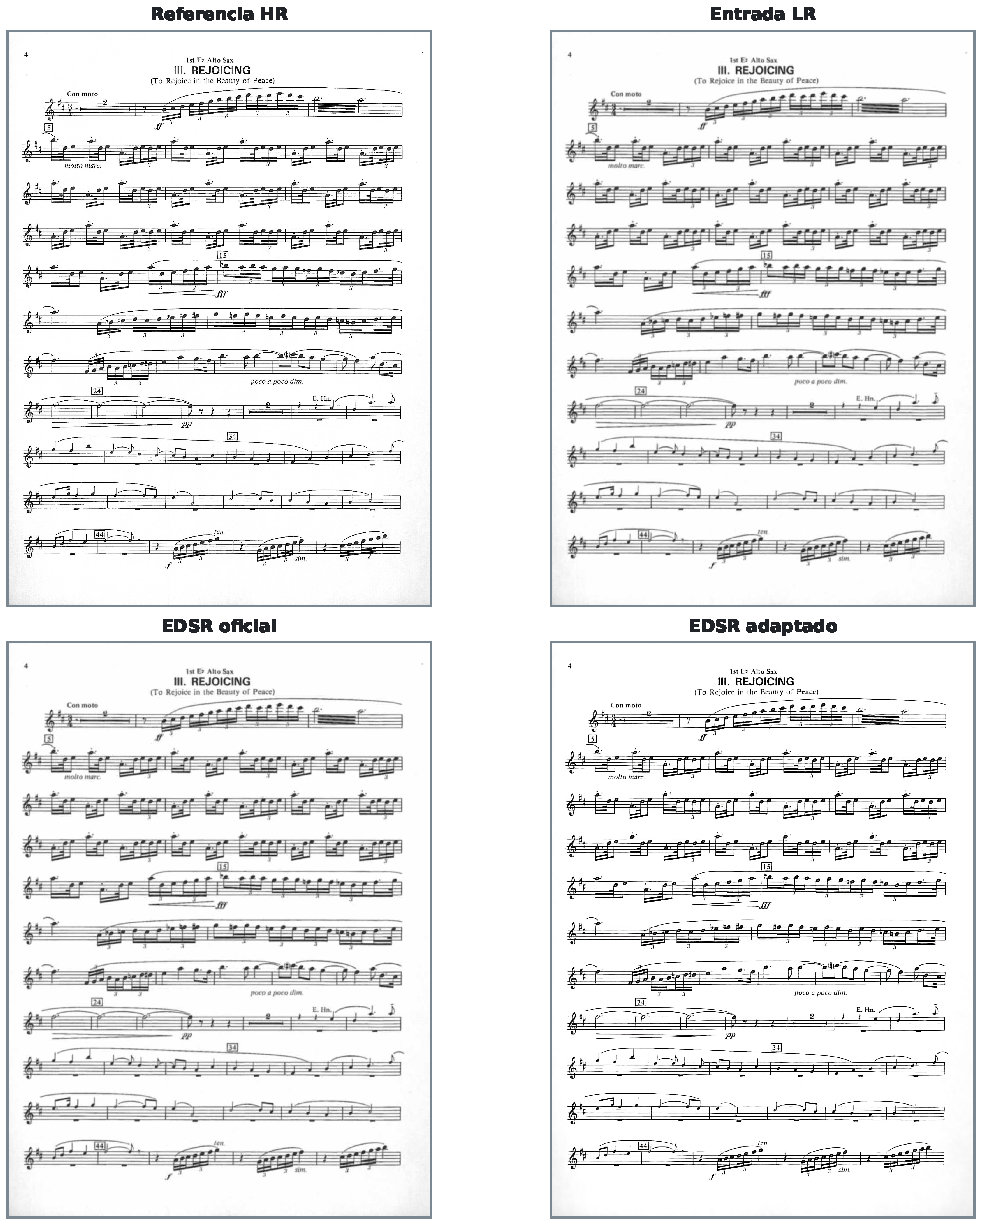
\includegraphics[width=\textwidth,height=0.82\textheight,keepaspectratio]{figures/results/external-accepted-full-page-x2-strong.pdf}
  \caption[Caso externo completo aceptado para consulta]{Caso externo fijo
  \texttt{three-revelations}, degradación \texttt{x2-strong}, aceptado para consulta. La salida
  adaptada mejora de forma visible la definición global frente al EDSR oficial, aunque texto y
  signos pequeños conservan daño procedente de LR. Extracto de una parte de saxofón alto primero en
  mi bemol de \emph{Three Revelations from the Lotus Sutra}, de Alfred Reed. Fuente: archivo musical
  de la Societat Joventut Musical d'Albal; página reproducida con autorización expresa para este
  TFG. La LR y las reconstrucciones son transformaciones de elaboración propia.}
  \label{fig:external-accepted}
\end{figure}

El rechazo \emph{Mari Carmen} aporta una condición documental distinta: notación de percusión
dispersa, cabezas no convencionales, tipografía fina y reducción x4 fuerte. El EDSR adaptado aumenta
el contraste respecto al oficial, pero no recompone con fiabilidad las cabezas, los matices y los
trazos más delgados. La baja densidad deja además pocos elementos redundantes que ayuden a
interpretar un símbolo degradado. Conservar este caso impide convertir once decisiones favorables
en una afirmación universal y fundamenta la vía profesional de rechazo del derivado.

\begin{figure}[p]
  \centering
  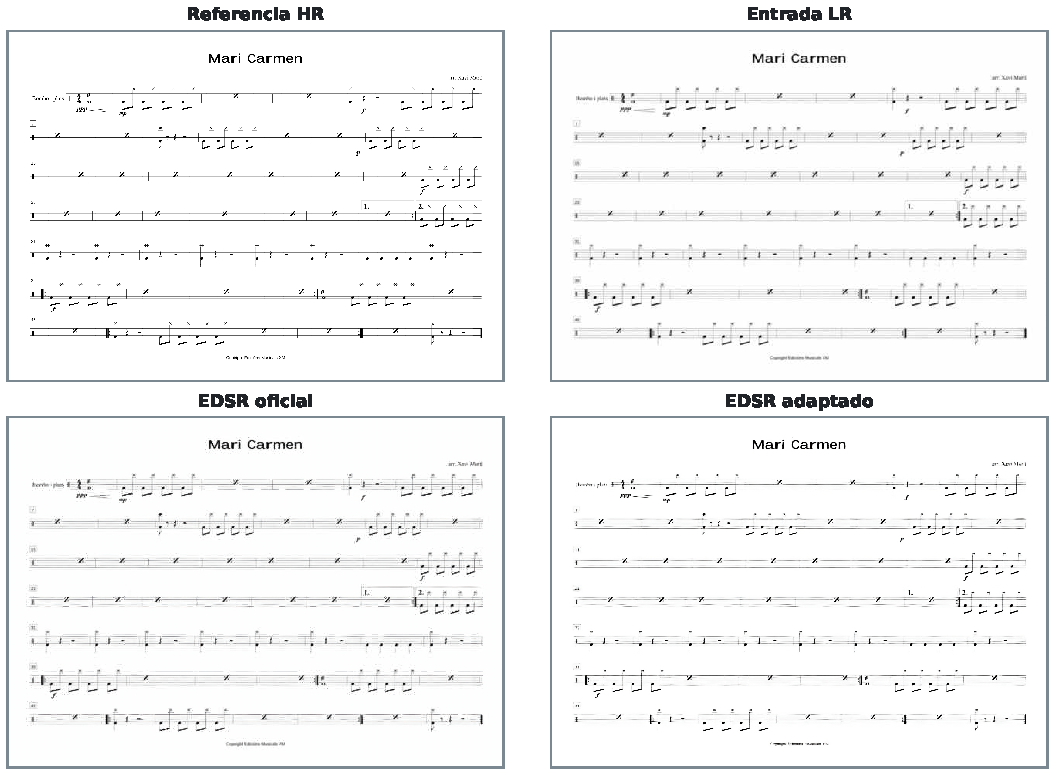
\includegraphics[width=\textwidth]{figures/results/external-rejected-full-page-x4-strong.pdf}
  \caption[Caso externo completo rechazado]{Caso externo fijo \texttt{mari-carmen}, degradación
  \texttt{x4-strong}, rechazado para consulta. El aumento de contraste del EDSR adaptado no recupera
  con suficiente fidelidad la notación fina de percusión perdida en LR. Extracto de la parte de
  bombo y platos de \emph{Mari Carmen}, arreglo de Xavi Martí. Fuente: archivo musical de la
  Societat Joventut Musical d'Albal; página reproducida con autorización expresa para este TFG. La
  LR y las reconstrucciones son transformaciones de elaboración propia.}
  \label{fig:external-rejected}
\end{figure}

La Figura~\ref{fig:external-details} permite inspeccionar tres situaciones de uso a mayor aumento:
una página aceptada, otra con reservas y la rechazada. En A se compara la limpieza de las notas
frente al EDSR oficial; en B, la separación entre los elementos sigue siendo una comprobación
necesaria aunque la página resulte globalmente consultable; en C, las cabezas y marcas finas de
percusión muestran por qué el aumento de contraste no basta: las cabezas en aspa de HR quedan
reducidas a manchas y no recuperan su geometría en las salidas. La decisión corresponde a la página
completa revisada, no solo al fragmento mostrado. Estos ejemplos complementan las doce páginas
completas e impiden confundir el aspecto de un detalle con una garantía de uso de toda la obra.

\begin{figure}[p]
  \centering
  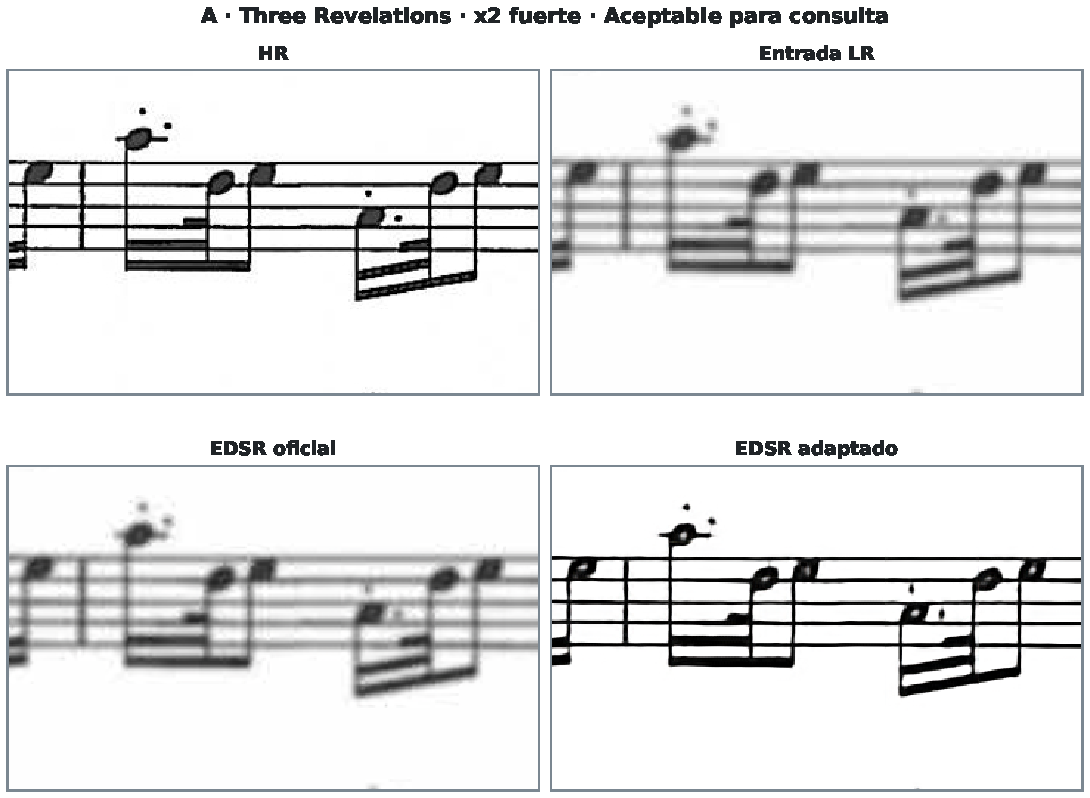
\includegraphics[page=1,width=\textwidth]{figures/results/external-detail-gallery.pdf}
  \caption[Ampliaciones de tres resultados del piloto externo]{Detalle de tres decisiones ya
  registradas, en tres láminas consecutivas. En esta primera, A: \emph{Three Revelations from the Lotus Sutra}, Alfred Reed, saxofón alto primero,
  x2 fuerte, aceptable para consulta. B: \emph{La rosa i el drac}, Francisco Valor, fliscorno
  segundo, x4 limpia, aceptable con reservas. C: \emph{Mari Carmen}, arreglo de Xavi Martí, bombo
  y platos, x4 fuerte, rechazado. Fuente: archivo musical de la SJMA; fragmentos reproducidos con
  autorización expresa para este TFG. LR y reconstrucciones son transformaciones propias;
  el encuadre se conserva dentro de cada caso y no se aplica realce adicional.}
  \label{fig:external-details}
\end{figure}
\clearpage

\begin{figure}[p]
  \centering
  \includegraphics[page=2,width=\textwidth]{figures/results/external-detail-gallery.pdf}
  \caption[B: caso externo con reservas]{Ampliación de La rosa i el drac, de Francisco Valor, fliscorno segundo, x4 limpia. La decisión de consulta con reservas corresponde a la página completa revisada. Fuente: archivo musical de la SJMA; reproducción autorizada para este TFG, con LR y reconstrucciones propias.}
\end{figure}
\clearpage

\begin{figure}[p]
  \centering
  \includegraphics[page=3,width=\textwidth]{figures/results/external-detail-gallery.pdf}
  \caption[C: caso externo rechazado]{Ampliación de Mari Carmen, arreglo de Xavi Martí, bombo y platos, x4 fuerte. Las cabezas en aspa de HR no recuperan su geometría. Fuente: archivo musical de la SJMA; reproducción autorizada para este TFG, con LR y reconstrucciones propias.}
\end{figure}
\clearpage


El demostrador local completó la carga validada de los dos puntos de control, el procesamiento por
teselas, la comparación original--derivado y la descarga PNG en sus pruebas automatizadas. En la
ejecución externa sobre CPU, la mediana por página fue de 25,8--26,4 segundos en x2 y de
10,3--10,6 en x4 para los dos EDSR. Esta inversión aparente se debe a que la entrada LR x2 contiene
más píxeles antes de reconstruir el mismo tamaño HR. El resultado es una prueba funcional local,
no una medición de usabilidad ni un servicio desplegado.

\clearpage
\section{Coste y comportamiento operativo}
La Figura~\ref{fig:runtime} resume la mediana por página en el dispositivo \texttt{cuda:0} de la
sesión Kaggle, que expuso dos Tesla T4 pero no ejecutó inferencia distribuida. Bicúbica
empleó entre 0,0038 y 0,0055 segundos; EDSR, entre 0,357 y 0,674; y SwinIR, entre 1,899 y 5,668.
SwinIR fue entre 5,2 y 8,5 veces más lento que EDSR y entre 486 y 1.045 veces más lento que
bicúbica, según la condición. Los tiempos \(\times 2\) fueron mayores porque la imagen de entrada
contiene más píxeles que en \(\times 4\) antes de reconstruir el mismo tamaño final.

A modo de escala operativa, procesar 1.000 páginas consecutivas bajo ese mismo entorno y sin contar
carga, descarga ni revisión supondría aproximadamente 4--6 segundos con bicúbica, 6--11 minutos con
EDSR y 32--95 minutos con SwinIR, según condición. Es una proyección aritmética del tiempo mediano,
no una prueba de rendimiento de un servicio: no incorpora concurrencia, memoria, colas ni
variabilidad entre documentos.

\begin{figure}[htbp]
  \centering
  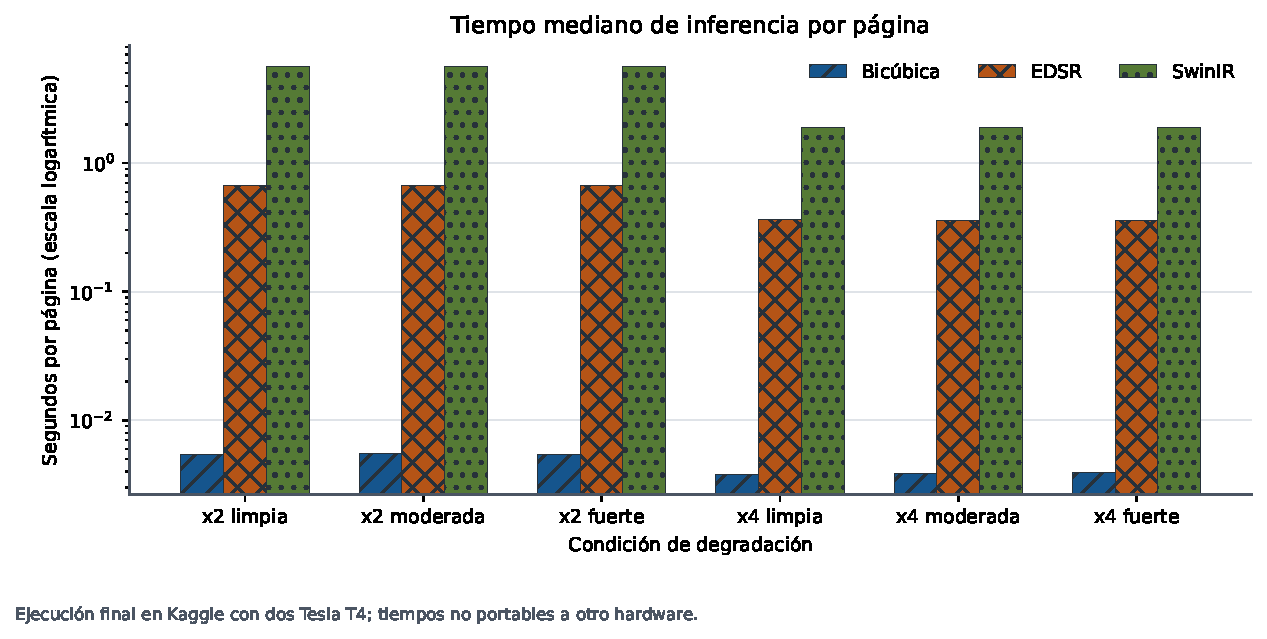
\includegraphics[width=\textwidth]{figures/results/runtime-median.pdf}
  \caption{Mediana del tiempo de reconstrucción por página en la ejecución Kaggle retenida. La
  escala vertical es logarítmica y los valores no se extrapolan a otro hardware. Fuente:
  elaboración propia.}
  \label{fig:runtime}
\end{figure}

El coste adicional de SwinIR solo queda justificado por fidelidad en las condiciones donde su
ventaja emparejada frente a EDSR fue clara. La ejecución no midió energía ni memoria máxima con una
instrumentación validada, por lo que no se atribuyen diferencias ambientales cuantitativas más
allá de hardware y duración.

\chapter{Validación y aplicación profesional}

\section{Validez dentro de las condiciones evaluadas}
\emph{Pendiente: triangular métricas, fallos de notación y recursos sin exceder la evidencia.}

\section{Escenarios profesionales y marco de decisión}
\emph{Pendiente: indicar métodos, condiciones, costes, precauciones y casos de no uso.}

\section{Aplicabilidad fuera del benchmark}
\emph{Pendiente: incorporar una ampliación realista o especialista solo si supera el gate; en caso
contrario, declarar la limitación y el trabajo futuro.}

\chapter{Conclusiones}

\section{Respuesta a los objetivos}
El objetivo general era determinar cuándo un conjunto pequeño de técnicas de superresolución puede
mejorar partituras digitalizadas sin convertir una reconstrucción visualmente convincente en una
afirmación falsa sobre su contenido. La comparación controlada responde que los modelos aprendidos
sí aumentan la fidelidad promedio frente a bicúbica, pero su utilidad depende de escala, severidad,
coste y revisión de los elementos musicales.

El estado del arte permitió separar interpolación, redes convolucionales, transformadores y métodos
perceptuales, y mostró que los resultados sobre imágenes naturales, documentos u OMR no demuestran
fidelidad musical. La auditoría de SMB conservó 685 elementos, identificó 260 grupos de fuente,
documentó 67 páginas no elegibles para comparación por sus anotaciones y preservó una muestra
principal intacta dentro de su única partición oficial. La degradación final definió seis condiciones normalizadas por
escala de pentagrama y la ejecución reconcilió 1.152 resultados sobre 64 obras independientes.

EDSR y SwinIR superaron a bicúbica en PSNR-Y y SSIM-Y para todas las condiciones. SwinIR destacó en
x2 limpia, x2 moderada y x4 limpia, pero EDSR igualó o superó su fidelidad en las condiciones más
difíciles y fue entre 5,2 y 8,5 veces más rápido. La revisión cualitativa halló símbolos alterados,
texto o dígitos corruptos y textura no natural en casos de ambas redes. La adaptación al dominio se
ejecutó después como estudio secundario sin reutilizar las 64 obras principales: el EDSR adaptado
mejoró al oficial en PSNR-Y y SSIM-Y en las seis condiciones sobre 20 obras nuevas, con intervalos
emparejados que no cruzaron cero. El resultado profesional es un marco condicionado en el que EDSR
preentrenado constituye la opción general por equilibrio entre fidelidad y coste, SwinIR una opción
selectiva y bicúbica una referencia rápida y transparente. La adaptación es prometedora cuando se
dispone de datos gobernados del dominio, pero no queda validada fuera de SMB ni como restauración
semántica.

En la revisión fija del modelo adaptado, cuatro de seis casos mostraron mejora sin defecto nuevo
claro y los dos casos fuertes conservaron daños ya presentes en LR. El ajuste redujo halos y
texturas y mejoró pentagramas y símbolos principales, pero no recuperó de forma fiable texto,
dígitos, alteraciones y otros elementos pequeños cuando la degradación había eliminado su
información. Por ello, su ventaja cuantitativa y visual no autoriza completar ni interpretar una
partitura sin cotejo humano.

La Tabla~\ref{tab:objective-evidence} cierra la trazabilidad entre lo prometido y lo entregado. El
ajuste fino se añadió únicamente después de asegurar el núcleo y se evaluó con un contrato separado
compatible con la integridad de la comparación principal.

\begin{table}[htbp]
  \centering
  \footnotesize
  \setlength{\tabcolsep}{3pt}
  \caption{Relación entre objetivos, evidencia y estado final. Fuente: elaboración propia.}
  \label{tab:objective-evidence}
  \begin{tabular}{p{0.31\textwidth}p{0.45\textwidth}p{0.14\textwidth}}
    \toprule
    Objetivo & Evidencia principal & Estado \\
    \midrule
    Estado del arte trazable & Síntesis crítica, fuentes primarias y criterios de selección & Cumplido \\
    Auditar y gobernar SMB & 685 registros, 260 obras, elegibilidad, licencias y hashes & Cumplido \\
    Predeclarar el experimento & Protocolo v2, muestra, pesos, métricas, semillas y reglas & Cumplido \\
    Comparar métodos emparejados & 1.152 resultados, intervalos, revisión fija y tiempos & Cumplido \\
    Evaluar adaptación acotada & 45/13/20 obras separadas; dos puntos de control y 360 resultados & Cumplido con límites \\
    Producir una guía profesional & Marco por condición, salvaguardas y casos de no uso & Cumplido con límites \\
    \bottomrule
  \end{tabular}
\end{table}

\section{Limitaciones, problemas y aprendizaje}
La principal desviación fue metodológica. El primer protocolo aplicó un desenfoque absoluto
calibrado sobre fragmentos sintéticos de pentagrama mayor. En páginas SMB completas, las condiciones
moderada y fuerte cambiaron de significado y algunas se volvieron destructivas. En lugar de
reinterpretar aquel resultado, se conservó como piloto de desarrollo, se normalizó el desenfoque
por la separación entre líneas, se seleccionaron 64 obras nuevas sin solapamiento y se repitió la
comparación completa. Esta corrección retrasó el trabajo, pero produjo una conclusión más sólida y
dejó una lección general: una degradación debe expresarse en relación con la estructura que pretende
modelar, no solo en píxeles de una muestra cómoda.

Las conclusiones se limitan a páginas SMB impresas con escala de pentagrama mensurable, a
degradaciones sintéticas y a los pesos exactos de EDSR y SwinIR. La adaptación comparte corpus y
generador de degradación entre sus roles, aunque mantenga obras disjuntas, y x4 alcanzó su mejor
validación en el límite de 2.500 pasos. Se revisaron cualitativamente seis páginas por estudio, por
lo que no se conocen tasas de fallo poblacionales. No hubo evaluación ciega por
especialistas, escaneos reales, manuscritos, medición de energía, OMR ni una tarea editorial. PSNR y
SSIM miden fidelidad de imagen, no corrección musical. La procedencia y los derechos por elemento
de SMB no están disponibles, lo que impide reproducir sus imágenes en la memoria.

El trabajo reforzó conocimientos de aprendizaje profundo, procesamiento de imagen, inferencia
estadística emparejada, diseño experimental y ejecución reproducible en entornos locales y
acelerados. También mostró el valor de conservar resultados negativos, separar exploración de
confirmación y traducir una métrica técnica en una decisión profesional con límites explícitos.

\section{Contribución y legado}
La contribución no es un nuevo modelo ni una aplicación desplegada. Es un protocolo reproducible
para estudiar superresolución de partituras, una corrección de degradación basada en escala de
pentagrama, una comparación emparejada con incertidumbre, una adaptación reproducible de EDSR, una
taxonomía de fallos musicales y un marco de decisión que incluye condiciones de no uso. Este conjunto permite a bibliotecas, archivos,
profesionales de patrimonio, intérpretes, investigadores y editoriales valorar una copia ampliada
sin confundirla con el original.

El legado técnico reside en el código Python, configuraciones congeladas, hashes de puntos de
control, manifiestos, semillas, pruebas, cuadernos y scripts de análisis. Un tercero con acceso
autorizado a SMB puede reconstruir el entorno, verificar las identidades y repetir el flujo. Los
artefactos generados conservan denominadores, resultados y limitaciones, pero no redistribuyen el
conjunto ni sus imágenes. EDSR se apoya en código MIT, SwinIR en Apache-2.0 y SMB se declara CC
BY-NC 4.0 a nivel de conjunto; cualquier reutilización debe revisar además los derechos de cada
fuente.

El efecto esperado es mejorar la toma de decisiones: favorecer copias de consulta reversibles,
conservar siempre el original y exigir cotejo humano cuando el resultado tenga consecuencias. El
protocolo también deja una base para extender la adaptación, estudiar escaneos reales u OMR sin
presentar esas líneas futuras como resultados ya validados.

\section{Relación con los estudios y competencias}
El TFG integra programación, visión por computador, aprendizaje profundo, tratamiento de datos,
estadística, gestión de proyectos y comunicación técnica. La contribución
individual comprende el análisis bibliográfico, el diseño experimental, la implementación y las
pruebas. También abarca las ejecuciones local y remota, la revisión visual, el análisis estadístico,
la interpretación profesional y la redacción. Elena Vázquez Barrachina, tutora del TFG, y Jorge
Calvo Zaragoza, director experimental, contribuyen conjuntamente a la orientación y revisión
integral del trabajo. Esta contribución no altera la autoría ni la responsabilidad individual
sobre las decisiones, la implementación y las conclusiones.

Respecto a las cinco competencias transversales vigentes, el compromiso social y medioambiental se
evidencia en el análisis de derechos, acceso al patrimonio, riesgo de información inventada y coste
computacional. La innovación y creatividad aparecen en la normalización por pentagrama, la
taxonomía de fallos y el marco condicionado de uso. El trabajo en equipo y liderazgo se concreta en
la responsabilidad individual, la coordinación explícita con la tutora y el director experimental,
y la trazabilidad de decisiones, sin atribuirles trabajo ejecutado por el estudiante. La
comunicación efectiva se desarrolla en la memoria, las figuras
y la futura defensa para un tribunal no especializado. La responsabilidad y toma de decisiones se
refleja en el bloqueo del benchmark, los protocolos previos, la corrección del error de degradación,
la apertura controlada de una adaptación secundaria, los \emph{NO-GO} restantes, la conservación
de resultados negativos y los límites explícitos.

\chapter{Trabajo futuro}

\emph{Pendiente: separar extensiones plausibles —escaneos reales, evaluación especialista, OMR,
PDF o aplicación— de las conclusiones ya validadas.}


\bibliographystyle{plain}
\bibliography{references}
\cleardoublepage

\APPENDIX
\chapter{Reproducibilidad y trazabilidad}

\emph{Pendiente: describir adquisición autorizada, entorno, configuraciones, ejecución, evaluación,
índice de evidencias y límites para que un tercero pueda obtener resultados similares.}


% El anexo ODS debe ser el último de la memoria.
\chapter{Relación del TFG con los Objetivos de Desarrollo Sostenible}
% Fuente única para el anexo incluido en la memoria y el fichero ODS independiente.
% Marcar exactamente una columna por fila con \textbf{X}.
% Categorías exigidas por la plantilla ETSINF: alto, medio, bajo y no procede.
\begin{center}
\resizebox{\textwidth}{!}{%
\begin{tabular}{|l|c|c|c|c|}\hline
\textbf{Objetivos de Desarrollo Sostenible} & \textbf{Alto} & \textbf{Medio} &
\textbf{Bajo} & \textbf{No} \\
& & & & \textbf{procede} \\ \hline
ODS 1. \textbf{Fin de la pobreza.} & & & & \textbf{X} \\ \hline
ODS 2. \textbf{Hambre cero.} & & & & \textbf{X} \\ \hline
ODS 3. \textbf{Salud y bienestar.} & & & & \textbf{X} \\ \hline
ODS 4. \textbf{Educación de calidad.} & & & \textbf{X} & \\ \hline
ODS 5. \textbf{Igualdad de género.} & & & & \textbf{X} \\ \hline
ODS 6. \textbf{Agua limpia y saneamiento.} & & & & \textbf{X} \\ \hline
ODS 7. \textbf{Energía asequible y no contaminante.} & & & & \textbf{X} \\ \hline
ODS 8. \textbf{Trabajo decente y crecimiento económico.} & & & & \textbf{X} \\ \hline
ODS 9. \textbf{Industria, innovación e infraestructuras.} & \textbf{X} & & & \\ \hline
ODS 10. \textbf{Reducción de las desigualdades.} & & & \textbf{X} & \\ \hline
ODS 11. \textbf{Ciudades y comunidades sostenibles.} & & \textbf{X} & & \\ \hline
ODS 12. \textbf{Producción y consumo responsables.} & & \textbf{X} & & \\ \hline
ODS 13. \textbf{Acción por el clima.} & & & \textbf{X} & \\ \hline
ODS 14. \textbf{Vida submarina.} & & & & \textbf{X} \\ \hline
ODS 15. \textbf{Vida de ecosistemas terrestres.} & & & & \textbf{X} \\ \hline
ODS 16. \textbf{Paz, justicia e instituciones sólidas.} & & & & \textbf{X} \\ \hline
ODS 17. \textbf{Alianzas para lograr los objetivos.} & & & & \textbf{X} \\ \hline
\end{tabular}%
}
\end{center}

\newpage

\section*{Reflexión}

La relación principal del TFG es con el ODS 9, Industria, innovación e
infraestructuras. El trabajo estudia la inteligencia artificial aplicada al patrimonio musical
digital y propone un procedimiento reproducible para decidir cuándo utilizarla. Incluye
degradación normalizada por escala de pentagrama, controles contra fugas de datos,
comparaciones emparejadas, revisión de fallos de notación y una guía profesional por
condición. Este componente metodológico y de innovación responsable justifica una relación alta,
sin desplegar un producto ni infraestructura de producción.

La relación con el ODS 11, Ciudades y comunidades sostenibles, es media. Su meta 11.4 contempla la
protección del patrimonio cultural \cite{un2030Agenda}, que incluye las partituras digitalizadas.
Una copia ampliada de consulta puede facilitar el acceso y reducir la manipulación del
original. La superresolución no conserva por sí misma un documento: puede alterar
símbolos, texto o trazos y generar una apariencia engañosa. Por ello, el uso recomendado mantiene
siempre la imagen original, identifica el derivado y exige cotejo humano cuando haya consecuencias
editoriales, interpretativas o de conservación. Se busca evitar confundir mejora visual y
restauración histórica auténtica.

El ODS 12, Producción y consumo responsables, tiene relación media. Se compararon
fidelidad y coste temporal: SwinIR fue entre 5,2 y 8,5 veces más lento que EDSR en la ejecución
retenida, sin ventaja general. Su uso indiscriminado habría consumido más recursos sin beneficio
consistente. El marco profesional propone EDSR como opción general y reserva SwinIR para las
condiciones donde su ganancia emparejada justifica el coste. También distingue el acceso a datos
de su reproducción: SMB se utiliza con acceso autorizado y no se redistribuye el corpus bruto;
la memoria incorpora comparaciones analíticas seleccionadas, atribuidas y con
transformaciones identificadas. Cada licencia y la base de publicación de cada imagen se consideran por
separado, sin presumir que el acceso autorice cualquier reproducción.

La relación con el ODS 13, Acción por el clima, es baja porque no se midió energía ni huella de
carbono con instrumentación validada. Se registraron hardware y duración y se limitaron modelos y
ejecuciones. Una comparación controlada, reutilizar código en local y Kaggle y acotar la adaptación
a un estudio secundario redujeron cálculo innecesario. Estas medidas ahorran recursos,
pero no permiten cuantificar un beneficio climático ni justifican una valoración mayor.

Los ODS 4 y 10 tienen relación baja e indirecta. Las copias de consulta podrían facilitar el
estudio de fuentes musicales a estudiantes, intérpretes o investigadores y mejorar el acceso a
material digitalizado de resolución insuficiente. El TFG no ha medido
aprendizaje, accesibilidad, cobertura geográfica ni reducción de desigualdades, y tampoco ha creado
un servicio público. La contribución es un escenario profesional futuro, no
impacto demostrado.

Los demás ODS no son aplicables. El
trabajo no aborda pobreza, alimentación, salud, género, agua, energía asequible, empleo, ecosistemas,
instituciones o alianzas mediante resultados directos. La innovación debe evaluarse junto con
sus riesgos: en patrimonio musical, un detalle falso puede ser
más perjudicial que una imagen borrosa porque parece fiable. La transparencia de las degradaciones,
los hashes, las licencias, los resultados negativos y los casos de no uso es
esencial para la responsabilidad social de la solución.


\end{document}
